\chapter{Stand van zaken}
\label{ch:stand-van-zaken}

% Tip: Begin elk hoofdstuk met een paragraaf inleiding die beschrijft hoe
% dit hoofdstuk past binnen het geheel van de bachelorproef. Geef in het
% bijzonder aan wat de link is met het vorige en volgende hoofdstuk.

% Pas na deze inleidende paragraaf komt de eerste sectiehoofding.

TO DO

\newpage
\section{Blockchain}
\label{sec:blockchain}
	\subsection*{Inleiding}
	In het eerste deel van dit hoofdstuk wordt de blockchain-technologie in haar basisvorm besproken. We beginnen met het introduceren  van  de verschillende concepten en principes waarop blockchain gebouwd is.  We doen dit door het bespreken van hetgeen \textcite{Swan2015} blockchain 1.0 noemt, ofwel de Bitcoin blockchain. In het paper Bitcoin: A Peer-to-Peer Electronic Cash System beschrijft de auteur, onder het pseudoniem Satoshi Nakamoto een monetair systeem dat niet verbonden is aan een bank of  andere financiële institutie. Satoshi Nakamoto is de oorspronkelijke ontwerper van de Bitcoin en richtte de eerste blockchain-database op. Tot op vandaag blijft de ware identiteit van deze persoon (of entiteit) een mysterie. Het paper werd gepubliceerd op 31 oktober 2008 en wordt vandaag gezien als het blockchain white paper,  de structuur die in \textcite{Nakamoto2008} beschreven wordt vormde de basis voor het wat men vandaag blockchain noemt.
	\subsection{Noodzaak}
			\subsubsection{Vertrouwen in de plaat van bewijs}
			\textcite{Nakamoto2008} start met de vaststelling dat het verkopen van waren en diensten op het internet zo goed als volledig afhankelijk is van grote financiële instituties die optreden als derde partij voor het verwerken van elektronische transacties. 
		
			Hoewel ons huidige betaalmodel naar behoren werkt voor de meeste transacties, kent het volgens de auteur van het paper, toch een inherent zwaktepunt: het is namelijk een systeem gebaseerd op vertrouwen en niet op bewijs.
			
			Transacties in het huidige systeem, zo stelt \textcite{Nakamoto2008}, zijn namelijk niet definitief, een pas uitgevoerde transactie is een veel gevallen nog omkeerbaar. Voor de financiële instellingen die fungeren als derde partij kan het ook niet anders: het is onvermijdelijk dat geschillen zullen optreden over bepaalde transacties. Bijgevolg is het ook onvermijdelijk dat er situaties zullen zijn waarin de instellingen via wie de transacties lopen moet ingrijpen door transacties ongedaan te maken. Omdat transacties in het huidige systeem niet als definitief kunnen beschouwd worden, is er een zekere graad van vertrouwen nodig om een transactie aan te gaan tussen de betrokken partijen.  Het aangaan van een transactie vergt daarom, vooral voor de ontvangende partij, een grotere nood aan vertrouwen. 
			
			Men geeft hier het voorbeeld van online-verkopers die zich genoodzaakt zien om hun klanten om meer persoonlijke informatie te vragen dan ze eigenlijk nodig hebben. En ook al worden er meer gegevens gevraagd dan nodig, dan nog is een zeker fraude percentage onvermijdbaar. 
		
			Wanneer men de analogie maakt voor gebruik van cash geld dan ziet men dat de bovenstaande problemen in veel mindere mate voorkomen. Bij het gebruik van cash geld gebeurt de transactie immers niet enkel op basis van vertrouwen maar vooral op basis van wederzijdse controle. Als een klant een bepaalt bedrag betaald of wisselgeld ontvangt dan telt deze het geld ter controle. Idem dito de ontvangende kant. Bij cash geld is het minder evident om een transactie ongedaan te maken. 
			
			Het paper komt tot de conclusie dat een alternatief elektronisch betalingssysteem nodig is. In zo’n systeem zouden transacties niet mogen gebeuren op basis van vertrouwen maar eerder basis van een wederzijdse controle, net zoals bij het voorbeeld van cashgeld- het geval was. Een controlemechanisme gebaseerd op crypto-grafisch bewijs zou twee partijen in staat kunnen stellen om online transacties rechtstreeks met elkaar aan te gaan, zonder daarbij gebruik te moeten maken van een vertrouwde partij. De noodzaak tot een 3e partij, in de vorm van een financiële instantie zoals een bank, is in een dergelijk systeem volledig geëlimineerd.
		
			In het systeem dat \textcite{Nakamoto2008} voorstelt zijn de transacties beschermt door cryptografie die het computationeel onpraktisch maakt om ze ongedaan te maken. De transacties zijn volledig onomkeerbaar en beschermen hiermee verkopers tegen fraude. Daarbovenop zijn borg-mechanismen, nodig om ook kopers beschermen, volgens de auteur ook makkelijk te implementeren in het systeem.
			
			\subsubsection{Het double-spending probleem}
			Het paper wijdt veel aandacht aan het oplossen van het dubble-spending probleem. Dit probleem beschrijft het bestaande risico dat bij een digitale vorm van geld of een ander digitaal-middel dezelfde middelen meerdere malen gespendeerd kunnen worden.
			
			Een van de fundamentele verschillen tussen contant en elektronisch geld is dat het eerste van een fysieke aard is. Dat betekend dat het geld tastbaar is, men draagt het bij zich, en men geeft het door wanneer men transacties maakt. Daarna is het geld weg. Eenmaal gespendeerd is contant geld op, hetzelfde geld kan elders niet opnieuw aangewend worden. Er is geen bank of andere financiële instantie voor nodig om dit verifiëren. Hoeveel men spendeert en hoeveel vermogen er nog rest is evident. 
			
			Bij elektronische vormen van geld is dit alles vele malen complexer. Ter verduidelijking nemen we hier het voorbeeld van een klassieke rekening bij een bank.
			
			\begin{figure}
				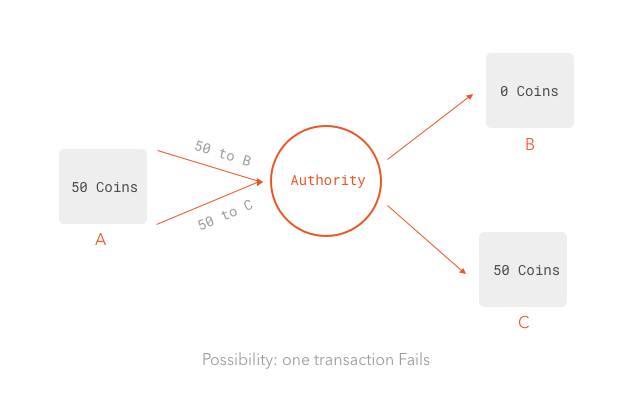
\includegraphics[width=\linewidth]{img/double_spending2.png}
				\caption{Double spending bemoeilijkt door een centrale autoriteit}
				\label{fig:double_spending2}
			\end{figure}
			
			Het geld op de hedendaagse bankrekening bestaat enkel en alleen als een elektronisch getal, een reeks van digitale cijfers bestaande uit 1’en en 0’en. Zo’n getal op zichzelf is gemakkelijk gewijzigd, men hoeft slechts wat 1’en en 0’en toe te voegen om een veelvoud van het oorspronkelijke te bekomen. Het is de bank die instaat voor de beveiliging van elektronisch geld. Waar de bank van weleer de bewaker was van vermogens in de vorm van kluizen of goudreserves, is de bank van vandaag de digitale bewaker van binaire vermogens.
			
			Bij een typische elektronische transactie tussen twee partijen vindt er geen transfer plaats van fysieke objecten, hetgeen er wel plaats vindt is aan de ene kat een verlaging van het elektronische vermogen van de eerste partij en aan de andere kant een verhoging van het vermogen van de tweede partij. 
		
			Gezien de enorme complexiteit die de beveiliging digitale systemen met zich meebrengt is het uitvoeren van elektronische transacties binnen het klassieke monetaire systeem altijd de verantwoordelijkheid van een vertrouwde derde partij geweest. Wanneer men een elektronische aankoop doet is het deze derde partij die een centrale autoriteit vormt wat betreft de veiligheid en de geldigheid van de transactie. Het is de vertrouwde derde partij die controleert op dubble-spending, vervolgens een bepaald bedrag in mindering breng van het oorspronkelijke vermogen en dit bedrag tenslotte toevoegt aan de kant van de verkoper. Dit wordt geïllustreerd in figuur \ref{fig:double_spending2}
			
			In de meeste gevallen neemt vertrouwde derde partij de vorm aan van een bank, maar alternatieve instanties die kunnen optreden als vertrouwde derde partij voor transacties. Voorbeelden hiervan zijn: PayPal, TransferWise, Google Pay en Apple Pay.
		
			Haalt men deze derde partij echter volledig uit het proces dan dringt de nood voor een compleet nieuwe oplossing voor het dubble-spending probleem zich onmiddellijk op.  Dit wordt geïllustreerd in figuur \ref{fig:double_spending1}
			
			\begin{figure}
				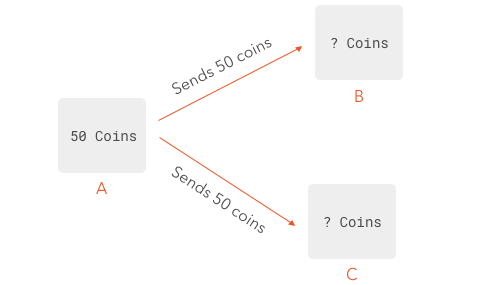
\includegraphics[width=\linewidth]{img/double_spending1.png}
				\caption{Double spending zonder een centrale autoriteit}
				\label{fig:double_spending1}
			\end{figure}
		
			Double-spending vormt een dusdanig groot probleem dat het de ontwikkeling van elektronisch geld zonder een vertrouwde autoriteit of een centrale server lange tijd onmogelijk werd geacht. In de volgende secties wordt de oplossing van \textcite{Nakamoto2008} voor het probleem besproken. 
			
			\subsubsection{Het Byzantijnse Generaalsprobleem}
			Het double-spending probleem is een probleem dat specifiek is voor digitale valuta. Het Byzantijnse Generaalsprobleem, is een gelijkaardig probleem, alleen is het van toepassing op een iets bredere context. Het byzantijnse vraagstuk omschrijft eigenlijk het achterliggende probleem bij double-spending: de vraag hoe men vertrouwen achterwege laat in een systeem zonder centrale autoriteit.
			
			Het probleem luidt als volgt: generaals van Byzantium moeten hun troepen coördineren voor een aanval, en dit op basis van berichten die ze elkaar versturen. De aanval moet met meer dan de helft van het totaal aantal troepen worden uitgevoerd op een exact moment, anders zal ze falen. Het is echter mogelijk dat een of meerdere generaals verraders zijn, die de aanval willen dwarsbomen. De identiteit van deze generaals kan niet achterhaald worden. De probleemstelling is dus hoe de generaals die te goeder trouw zijn toch hun troepen kunnen coördineren tot een aanval, vrij en open met elkaar communicerend, zonder dat een verrader hun plannen kan dwarsbomen door valse berichten te versturen. Het Byzantijnse Generaals probleem wordt geillustreerd door figuur \ref{fig:byzantium}
			
			Het Byzantijnse generaalsprobleem is tot op vandaag erg relevant omdat het van toepassing is op eender welke context waarin communicatie tussen verschillende entiteiten een cruciale rol speelt en er geen absoluut vertrouwen is. Het gebied van gedistribueerde computernetwerken is hier een perfect voorbeeld van. De oplossing van \textcite{Nakamoto2008} claimt niet alleen het double-spending probleem op te lossen, maar ook het byzantijnse generaals probleem. Men spreekt ook wel van een model met Byzantijnse fouttolerantie.
			
			\begin{figure}
				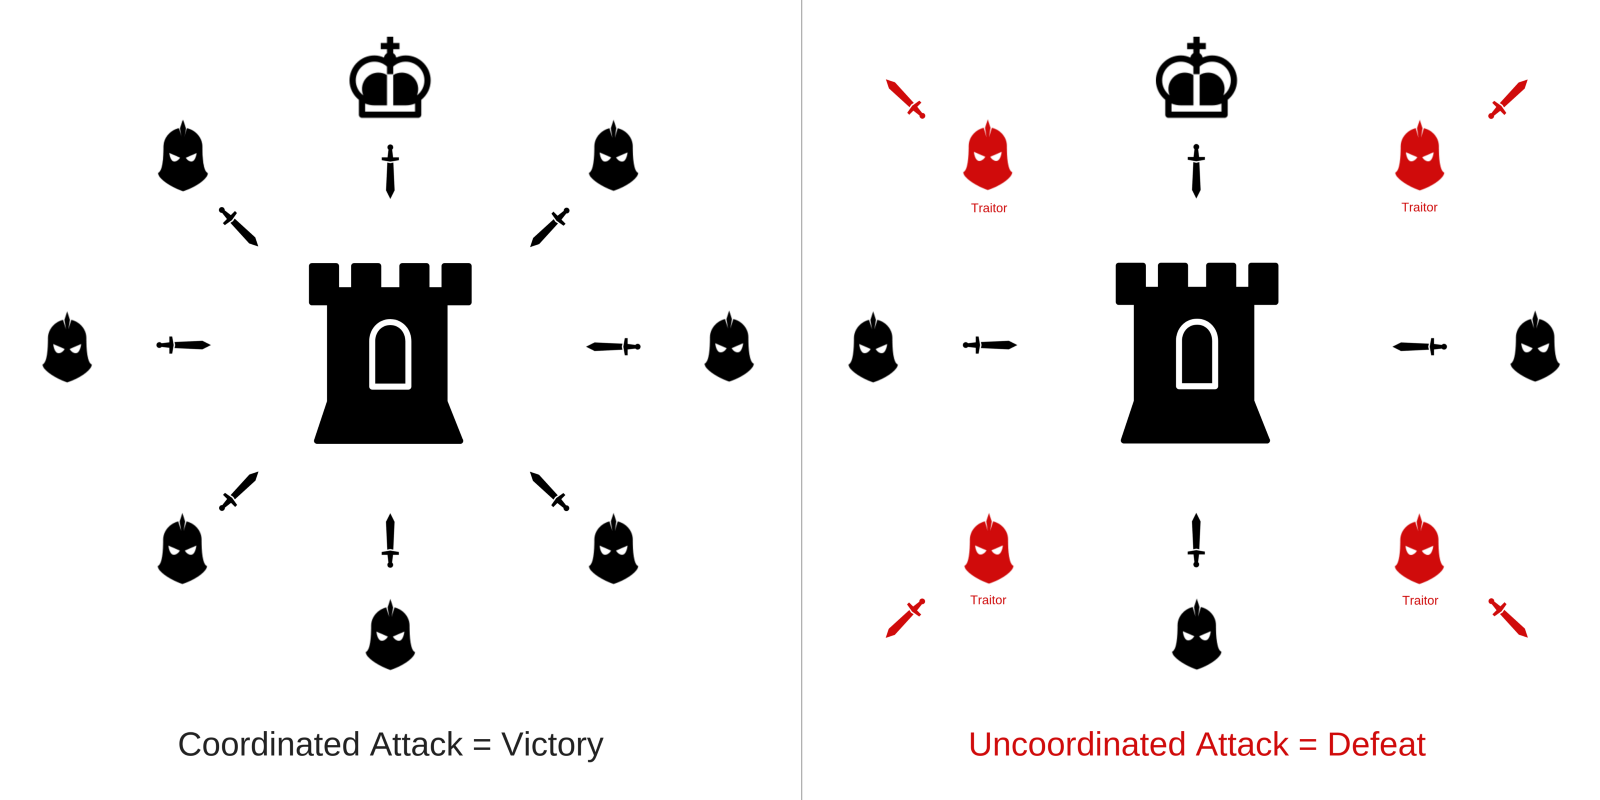
\includegraphics[width=\linewidth]{img/byzantine_generals.png}
				\caption{Het Byzantijnse generaals probleem.}
				\label{fig:byzantium}
			\end{figure}
			
	\subsection{Transacties}
	Het monetaire systeem dat \textcite{Nakamoto2008} voorstelt werkt op basis van digitale munten. Deze munten worden gedefinieerd als ketens opgebouwd uit digitale ondertekeningen. Als de eigenaar van zo’n een munt een transactie aangaat wordt de munt doorgegeven aan de volgende eigenaar door ze digitaal te ondertekenen met een hash. Deze hash bestaat uit de hash van de vorige transactie gecombineerd met de publieke sleutel die de volgende eigenaar identificeert. De nieuwe hash wordt aan de keten van ondertekeningen toegevoegd waaruit de munt bestaat. De ontvanger kan dan de ondertekeningen, en daarmee historiek van eigendom van de munt verifiëren. 
			
	De historiek van een digitale munt kennen lost het dubble-spending probleem echter niet op. Men kan immers niet controleren of dezelfde munt niet ergens anders werd aangewend. \textcite{Nakamoto2008} stelt dat er een manier nodig is om voor iedere munt te verifiëren dat de vorige eigenaar geen eerdere transacties met de munt heeft aangegaan. Daartoe beslist men om de chronologisch eerst-voorkomende transactie van een eigenaar met een munt als valabel te beschouwen en alle daaropvolgende transacties van die eigenaar als double-spending. 
			
	Om de chronologische orde van een transactie te kunnen bepalen, is er kennis nodig van alle transacties. De enige manier om dit zonder vertrouwde partij te doen is door alle transacties publiek aan te kondigen. Vervolgens is er een mechanisme nodig waarbij alle participanten van het systeem (alle computers binnen het netwerk), hierna nodes genoemd, gezamenlijk kunnen beslissen over de exacte volgorde waarin transacties gebeurden. \textcite{Nakamoto2008} stelt voor om het probleem op te lossen startend vanuit een timestamp server. 
			
	\subsection{Timestamp Server}
	Een digital timestamp is een digitaal certificaat dat verzekerd dat een digitaal document op een bepaald ogenblik bestond. Er zijn meerdere, zeer specifieke technieken om betrouwbare digitale timestamps te kunnen produceren. In het algemeen zijn deze technieken onder te verdelen in twee grote categorieën: degene die gebaseerd zijn op een vertrouwde derde partij en degene die gebaseerd zijn op gedistribueerd vertrouwen. (BRON: https://nakamotoinstitute.org/static/docs/secure-timestamping-service.pdf )
	
	In dit geval wordt door de auteur er door \textcite{Nakamoto2008} gekozen voor de gedistribueerde techniek. In de volgende subsectie wordt een methode besproken om niet langer op basis van vertrouwen te werken.
	
	\textcite{Nakamoto2008} stelt voor om een timestamp server te gebruiken om de chronologische ordening van transacties die gebeuren met zijn digitale munt te bepalen.  Concreet werkt deze timestamp server door meerdere transacties die een timestamp moeten krijgen samen te nemen in een blok, er een hash van te berekenen en deze vervolgens openbaar te maken. (insert foto uit white paper)
	
	De timestamp bewijst het bestaan van de items op dat specifieke moment, gezien deze verwerkt zijn in de hash, en de hash uniek is en alleen maar kon gegenereerd worden uit specifieke combinatie van items. De timestamp bevat verder ook de voorafgaande timestamp in de hash, waardoor een ketting ontstaat. Iedere timestamp versterkt daarbij de voorafgaande, een chronologische historiek van transacties ontstaat.
	
	De reden dat men hier van een gedistribueerde techniek spreek is omdat de keten van transactie blokken niet op een centraal punt bestaat. Er bestaat een exemplaar van de database-structuur, met alle informatie erin op iedere node van een peer-to-peer netwerk. 
	
	Een peer-to-peer netwerk is een netwerk bestaande uit onderling verbonden computers waarbinnen iedere computer gelijkwaardig is en er dus geen sprake is van centrale autoriteit. 
	
	Het netwerk in zijn geheel wordt gebruikt als timestamp server om bewijs te genereren van de chronologische volgorde van transacties. Iedere node van het netwerk kent de volledige historie van transacties en kan de validiteit van gemaakte transacties bewijzen. Een partij die een frauduleuze transactie probeert te plegen valt snel door de mand gezien ze slechts 1 node in het netwerk representeert. Alle andere nodes leveren immers een bewijs dat afwijkt van dat van de frauduleuze node. Het netwerk accepteert periodiek een aantal transacties tegelijkertijd, deze vormen een zogenaamd blok. Blokken waarover er een consensus van 50\% of meer is worden geaccepteerd en in alle nodes aan een interne keten van blokken toegevoegd.
	
	Een database systeem, waarbij informatie periodiek in blokken geaccepteerd wordt en in iedere node van een P2P netwerk wordt toegevoegd aan een keten van blokken, noemt men vandaag de dag een blockchain.
	
	Een blockchain kan als veilig beschouw worden zolang minstens 50\% van de rekenkracht van het netwerk niet gecomprimeerd is, en het merendeel van de bewijzen dus steeds de waarheid representeert. In praktijk betekent dit een systeem dat nagenoeg oncomprimeerbaar is. In het geval van het hedendaagse Bitcoin netwerk spreekt men bijvoorbeeld van een netwerk met rond de 10.000 nodes (LaTex Bron Vermelden). Om succesvol te frauderen zouden aanvallers van het Bitcoin netwerk maar liefst de helft van al deze computers, verspreid over heel de wereld moeten controleren. 
			
	\subsection{Proof-of-Work}
	\label{subsec:pow}
	Om een gedistribueerde timestamp server op peer-to-peer basis te laten werken is er een extra veiligheidsmechanisme nodig dat het berekenen van hashes opzettelijk moeilijker maakt zodat het langer duurt om een blok toe te voegen. 
	
	Het concept, dat door \textcite{Nakamoto2008} proof-of-work genoemd wordt, is essentieel omdat moderne CPU’s over enorme rekenkracht beschikken. Mits er geen extra veiligheidsmechanisme zou zijn zouden hashes zeer snel berekent kunnen worden. Zodanig snel dat het mogelijk zou zijn voor een enkele aanvaller om een aanpassing te maken in de ketting en voor alle volgende blokken de hashes te opnieuw te berekenen. 
	
	Naargelang de ketting groeit en er meer hashes gebaseerd zijn op een voorgaande hash wordt het door proof-of-work steeds moeilijker om gegevens te wijzigen. Immers: een wijziging van gegevens betekent dat de hash ook herrekend moet worden. Dit veroorzaakt corruptie van de hashes van alle daaropvolgende blokken, de enige manier om dit op te lossen is de hashes van iedere blok te herrekenen. 
	Gezien de gemiddelde proof-of-work echter 10 minuten duurt en er ook om de 10 minuten een nieuwe blok aan de keten wordt toegevoegd is het bijna onmogelijk dat de corruptie niet door andere nodes wordt opgemerkt.
	
	Concreet bestaat de proof-of-work eruit dat er moet gezocht worden naar een bepaalde waarde. De waarde moet aan een voorwaarde voldoen: als men de hash functie toepast op de waarde dan moeten de eerste x aantal bits van het resultaat een 0 zijn. 
	
	De aard van een hashfunctie laat niet toe om aan reverse-engineering te doen, of anders gezegd men kan niet van een resultaat beginnen dat aan de voorwaarden voldoet om zo de gevraagde waarde te vinden. Proof-of-work kan dus alleen geleverd worden door miljarden waarden te overlopen, er de hash-functie op toe te passen en te controleren of er aan de voorwaarde voldaan is. Het is met andere woorden zeer tijdsconsumerend rekenwerk. De gemiddelde tijd nodig om een hash te vinden is exponentieel in x (het gevraagde aantal start-bits van de hash die 0 zijn).
	
	Zoals vermeld wordt het accepteren van nieuwe blokken gedaan op basis van een meerderheids-stem. Een vraag die hier opkomt is wat er precies als stem moet tellen en wat niet. Als de meerderheid bijvoorbeeld bepaald zou worden aan de hand van een zogenaamd one-ip-address-one-vote model dan zou het systeem misbruikt kunnen worden door nodes meerdere IP-adressen te laten alloceren. Proof-of-work biedt hier de oplossing. De meerderheidsbeslissing wordt gerepresenteerd door de langste keten, dewelke waarin de langste proof-of-work tijd geïnvesteerd is. Zolang de meerderheid van de CPU-kracht in het netwerk gecontroleerd wordt door oprechte nodes, zal deze ketting sneller groeien dan enige andere ketting. In essentie is het een one-CPU-one-vote model ~\autocite{Nakamoto2008}.
	
	Om te compenseren voor toenemende hardware-capabiliteit wordt de moeilijkheid van de proof-of-work dynamisch bepaald door een bewegend gemiddelde dat er op gericht is om het aantal blokken dat per uur toegevoegd wordt constant te houden. Als hashes te snel worden gegenereerd, wordt de moeilijkheid simpelweg verhoogd ter compensatie. 
	\subsection{Netwerk}
		\subsubsection{Verwerking  van transacties}
		In deze paragraaf wordt een abstracte schets gegeven van de conceptuele werking van \textcite{Nakamoto2008}’s netwerk:
		\begin{enumerate}
			\item Transacties worden gebroadcast naar ieder node in het netwerk
			\item Binnenkomende transacties worden in een blok gegroepeerd door iedere node.
			\item Iedere node werkt om de proof-of-work op te lossen
			\item De node die de proof-of-work als eerste vindt broadcast de blok van transacties zoals gekend door die node naar alle ander nodes.
			\item Al de andere nodes accepteren dit blok, op voorwaarde dat de bevatte transacties geldig zijn en niet double-spent.
			\item Nodes bevestigen hun acceptatie door aan de creatie van het volgende blok te beginnen, gebruik makende van de hash van het vorige blok.
		\end{enumerate}
		\subsubsection{Langste ketting}
		Het is steeds de langste ketting die als de correcte wordt beschouwd en verder wordt uitgebreid. Als twee nodes gelijktijdig een verschillend blok broadcasten dan zullen sommige nodes de ene versie eerst ontvangen en andere nodes de andere. Er ontstaat dan een situatie waarin er twee verschillende versies van de keten zijn binnen het netwerk. Deze discrepantie wordt pas weggewerkt wanneer de volgende proof-of-work wordt geleverd en er een weer een langste ketting is. Nodes die op de andere alternatieve keten werkten, schakelen weer over naar de ware keten.
		\subsubsection{Fout-tolerantie}
		Het systeem kent een hoge fout-tolerantie, het kan overweg met vrij veel fouten die zich in een realistisch scenario  kunnen voordoen binnen een netwerk. Zo kan het best zijn dat de broadcast van een nieuwe transactie niet iedere node in het netwerk bereikt. Dit is geen probleem zolang het merendeel van de nodes de transactie wel ontving. Hetzelfde geld voor de broadcasts van blokken, als een node door bepaalde omstandigheden een broadcast van een blok niet ontvangt, zal de node bij de volgende broadcast realiseren dat het dat blok mist en het netwerk verzoeken om dit door te sturen.
	\subsection{Mining}
		\subsubsection{Nieuwe bitcoins}
		Gezien er voor de bitcoin geen centrale autoriteit is die het geld maakt of verdeeld is er een alternatieve wijze nodig om de digitale munten te creëren en in circulatie te brengen. Een analogie voor de creatie van nieuwe bitcoins, zo stelt \textcite{Nakamoto2008}, is het mijnen van een kostbare grondstof zoals goud. Bij de goud-mijnbouw moet er grote hoeveelheden middelen besteed worden om nieuw goud te ontginnen en in circulatie te brengen. Bij bitcoin is de situatie vergelijkbaar. De creatie van iedere bitcoin, hoewel enkel digitaal, vergt een zekere prijs in tijd en in middelen, met name elektriciteit.
		
		Conventie in het bitcoin netwerk is dat de eerste transactie van ieder blok een speciale transactie is, die een munt toekent aan de eigenaar van het blok. Het idee hier is om een stimulans te creëren die nodes ertoe aanzet om aan proof-of-work te doen en zo het netwerk te ondersteunen. De periodieke creatie van iedere blok is dus eigenlijk een race tussen duizenden nodes van het netwerk om als eerste de proof-of-work te kunnen leveren en in ruil daarvoor een beloning in bitcoin te ontvangen. 
		
		De analogie die \textcite{Nakamoto2008} maakt tussen bitcoin en mijnbouw, leidde tot de hedendaagse benaming voor dit concept: mining. 
		
		\subsubsection{Transacties}
		De stimulans om het netwerk te ondersteunen zal deels gecreëerd worden aan de hand van transactie kosten. \textcite{Nakamoto2008} stelt dat als de output waarde van een transactie minder is dan de input waarde, het verschil een transactie kost is die toegevoegd wordt op de stimulanswaarde van het blok dat de transactie bevat. Hiermee wordt bedoeld dat de nodes van het netwerk niet alleen bitcoin verdienen door het creëren van nieuwe bitcoins maar ook door het verwerken van transacties. Dit is van fundamenteel belang gezien het totaal ‘ontginbare’ bitcoins eindig is. Eenmaal een aantal bitcoins in omloop is zullen er geen nieuwe bitcoins meer gecreëerd kunnen worden en zal de ondersteuning van het netwerk overschakelen naar volledige financiering door middel van transactie kosten, deze zullen volgens \textcite{Nakamoto2008} op hun beurt stabiliseren en inflatievrij\footnote{De Bitcoin is sinds haar creatie steeds onderhevig geweest grote fluctuaties, zie https://bitcoinfees.info/} worden.
		
		De stimulans kan ook helpen om nodes eerlijk te houden. Zo zal de potentiële aanvaller van het netwerk ondervinden dat de CPU kracht, nodig om fraude te plegen, veel lucratiever blijkt wanneer aangewend voor eerlijke mining-doeleinden. 
		
		
		
	\subsection{Disk Space}
		\subsubsection{Hash-boom}
		\textcite{Nakamoto2008} stelt  een manier voor waarop data van oude transacties kan verwijderd worden om opslag ruimte te besparen. Om een dergelijke actie mogelijk te maken, zonder dat de hash corrumpeert, worden transacties binnen ieder blok in een structuur opgeslagen die men een hash-boom noemt. Zo’n structuur stelt instaat om de onderliggende transactie data te verwijderen maar de hashes te behouden.
		
		\subsubsection{Wet van Moore}	
		\textcite{Nakamoto2008} stelt dat gezien de Wet van Moore voorspelt dat hardware capaciteiten per jaar veel sneller zullen blijven toenemen dan de opslagruimte nodig om de groeiende keten van blokken in te bewaren, miners zich eigenlijk geen zorgen zouden moeten maken over opslagruimte. De Wet van Moore wordt geïllustreerd door figuur \ref{fig:moore}.
		\begin{figure}
			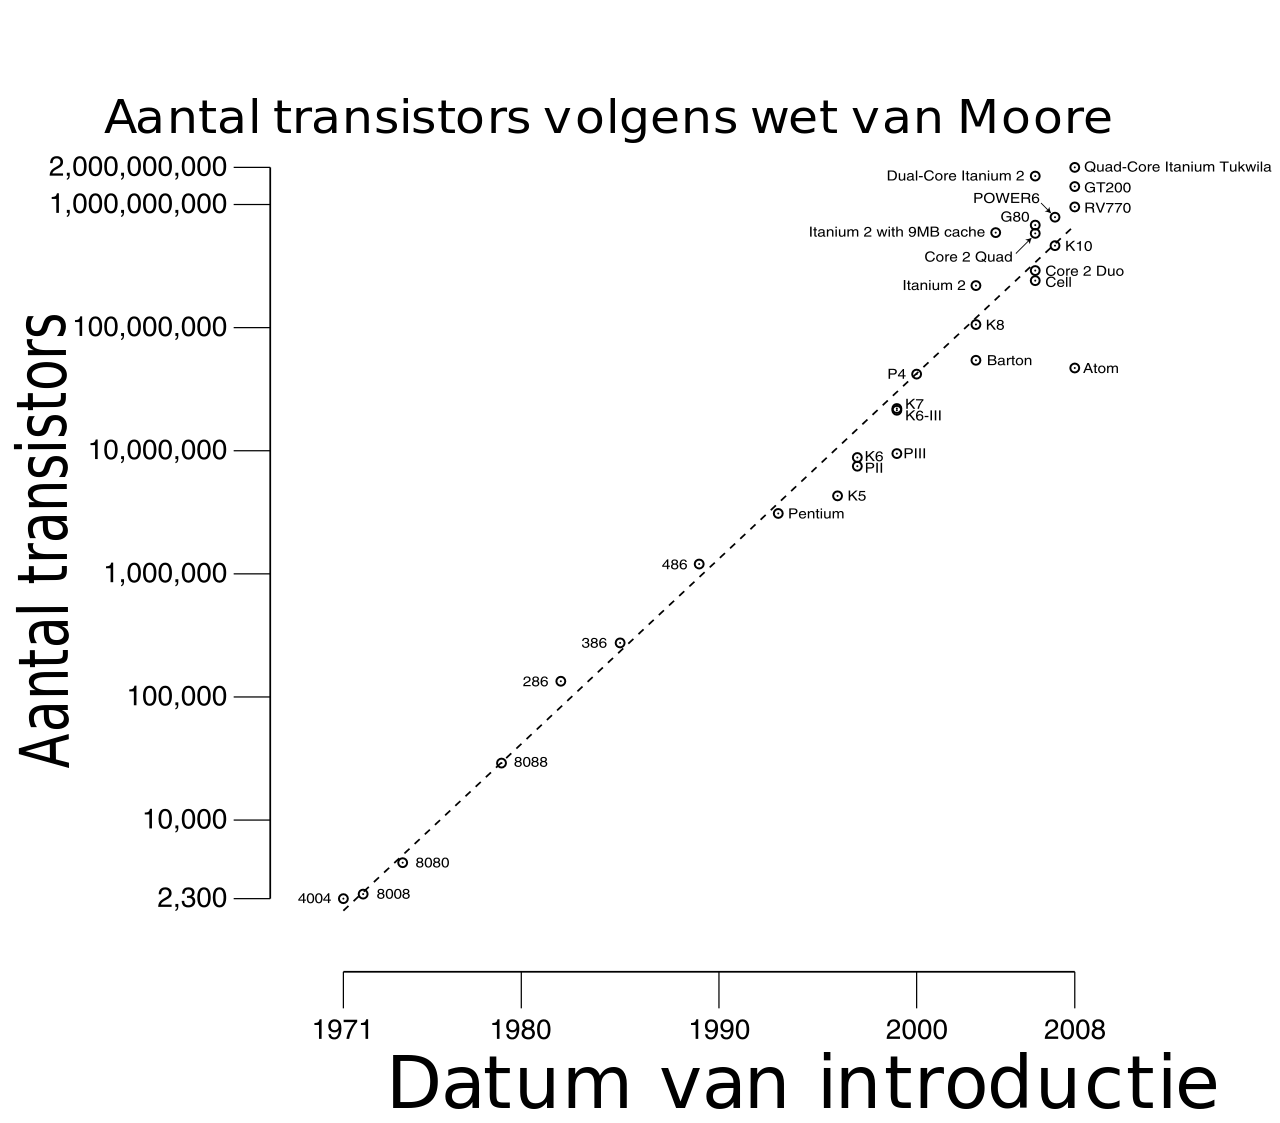
\includegraphics[width=\linewidth]{img/moore.png}
			\caption{De Wet van Moore.}
			\label{fig:moore}
		\end{figure}
		
		\subsection{Simpelere Verificatie van Betaling}
		Volgens \textcite{Nakamoto2008} is het mogelijk om betalingen te verifiëren zonder de hulp van een volledige netwerk-node, die iedere blok ooit gecreëerd kent. Om een transactie te verifiëren moet een gebruiker enkel een kopie hebben van de headers van alle blokken uit de langste keten. Deze kunnen alleen verkregen worden door de netwerk-nodes te bevragen en op een gegeven te beslissen dat men de langste keten gevonden heeft, en vervolgens van deze keten de tak van de hash-boom die de transactie aan het blok linkt te nemen.
	
		Met deze hash-tak kan de gebruiker wel is waar niet de transactie zelf controleren, maar er kan aan de hand van de positie van de hash van de transactie wel gecontroleerd worden of de transactie al geaccepteerd is door de node en het netwerk.
		
		Op deze manier is verificatie gemakkelijk, zolang eerlijke nodes controle over het netwerk hebben. Nodes kunnen transacties altijd zelf verifiëren, maar de vereenvoudigde methode kan beetgenomen worden door aanvallers die meer dan de helft van het netwerk controleren. Een mogelijke strategie hiertegen zou zijn om de volledige keten te downloaden wanneer er een ongeldige blok binnenkomt. 
	\subsection{Combineren en splitsen van transacties}
	Opdat er geen aparte transactie voor iedere munt die van eigenaar wisselt zou moeten gemaakt worden, voorziet \textcite{Nakamoto2008} een systeem waarin transacties gecombineerd en gesplitst kunnen worden. Zo kan men bijvoorbeeld drie Bitcoins in een enkele transactie versturen, maar ook 0.5 Bitcoin als wisselgeld ontvangen.
	
	Om dit moglijk te maken wordt er gewerkt met een systeem van inputs en outputs. Een transactie kan een of meerdere inputs hebben en een of twee outputs. De inputs stellen de bron(nen) waar het geld vandaan komt voor, eenderwelke waarde in bitcoin kan hier meegegeven worden. De output stellen de ontvangende kant voor, de eerste output is de waarde voor de ontvanger, de tweede output is optioneel en is voor het eventuele wisselgeld dat de verzender kan ontvangen.
	\subsection{Privacy}
	In het traditionele monetaire systeem ligt alle kennis over transacties bij de financiële instituties. De bank, als vertrouwde derde partij kan gemakkelijk privacy creëren door de toegang tot informatie over een transactie te limiteren tot de betrokken partijen. 
	
	In het model dat we vanaf nu de blockchain zullen noemen, is deze methode onmogelijk door de noodzaak tot het publiek aankondigen van transacties over het hele netwerk.  \textcite{Nakamoto2008} stelt echter dat privacy wel enigszins kan behouden worden door informatie op een ander plaats te beperken. Men stelt voor om de publieke sleutels, die bitcoin-portefeuilles identificeren anoniem te houden, en er dus geen naam aan te koppelen. Op deze manier mag iedereen dan wel kunnen zien welke transacties er plaats vinden, maar door de anonimiteit van zender en ontvanger wordt privacy grotendeels gegarandeerd.
	
	Om de privacy nog te verbeteren zou men ook kunnen opteren voor een systeem waarin iedere gebruiker per transactie een nieuwe sleutel krijgt die uniek identificerend is. Voor transacties met meerdere inputs is er echter geen manier om te verbergen dat de inputs van een eigenaar afkomstig zijn.
	\subsection{Nakamoto’s Conclusie}
	In het paper presenteert men een nieuw systeem voor elektronische transacties. Men start vanuit munten die opgemaakt zijn uit digitale ondertekeningen. Vervolgens lost men het double-spending probleem op. Om dit te doen wordt er een peer-to-peer netwerk voorgesteld dat gebruik maakt van zogenaamde proof-of-work om de historiek van gemaakte transacties op te slaan. 
	
	De implementatie van dit alles is een aard die het computationeel onpraktisch maakt om het systeem aan te vallen voor frauduleuze doeleinden. Het beslaat immers een robuust netwerk met weinig tot geen complexe structuur, maar waar door anonimiteit de privacy grotendeels gerespecteerd blijft. 
	
	Nodes binnen het netwerk werken allemaal tegelijk, doch zonder enige coördinatie of afhankelijkheid. Ze kunnen het netwerk verlaten en zich naar believen weer vervoegen. Nodes die zijn weggeweest moet enkel de volgende proof-of-wok accepteren om weer helemaal mee te zijn met alles wat er gebeurd is. 
	
	Er wordt gestemd op basis CPU-kracht: accepteren van blok gebeurt door aan de proof-of-work te beginnen werken, afwijzen van een blok gebeurt door dit te weigeren. Op basis van dit consensus mechanisme kunnen extra regels afhankelijk voor een der welke usecase worden toegevoegd ~\autocite{Nakamoto2008}. 
	\newpage
\section{Ethereum en smart contracts}
\label{sec:ethereum-en-smart-contracts}
	\subsection*{Inleiding}
		In het tweede deel van dit hoofdstuk wordt een beeld geschetst van wat \textcite{Swan2015} blockchain 2.0 noemt, ofwel 'Blockchain voorbij Bitcoin'. De concepten die in het vorige hoofdstuk werden besproken vormen de basis van de blockchain technologie. De Bitcoin blockchain staat intussen echter al weer een stuk verder en de Bitcoin is ook bijlange na niet meer de enige cryptomunt. De Bitcoin blockchain is dus bijlange niet meer de enige blockchain. Concreet wordt er in dit hoofdstuk dieper ingegaan op het concept  smart contracts, vervolgens wordt er ook een overzicht gegeven van Ethereum. Dit alles wordt uitgebreid besproken omdat het van belang zal worden eenmaal we blokchain stemsystemen (zie \ref{sec:blockchain-gebaseerd-stemmen}) bespreken.
	\subsection{Noodzaak}
		\subsubsection{Wat  zijn smart contracts?}
			Smart contracts zijn een concept dat de blockchain-technologie een stap verder neemt. In \textcite{Swan2015} worden ze omschreven als gedecentraliseerde contracten die niet langer een autoriteit (zoals een rechtbank) nodig hebben. Het zijn in feite digitale contractprogramma’s die zichzelf kunnen valideren en uitvoeren wanneer aan bepaalden voorwaarden is voldaan. Ook hier bestaat het concept sinds de jaren negentig ~\autocite{Szabo1996}. Bij het lezen van \textcite{Nakamoto2008} is het duidelijk dat er vanaf het prille begin van de bitcoin een visie was om een dergelijke systeem te implementeren. Blockchain-technologie staat immers niet alleen toe om data op te slaan, ook programma’s kunnen in de blockchain worden opgeslagen. Smart contracts vormen de basis van de nieuwe Blockchain 2.0 van vandaag, zowat iedere grote blockchain-speler probeert ze te implementeren~\autocite{Swan2015}.
		\subsubsection{Wat is Ethereum?}
			Ethereum (figuur \ref{fig:ethereum}) is een opensource-platform dat werd opgericht in 2015. Net zoals bitcoin maakt het gebruik van een gedecentraliseerd netwerk, gebaseerd op het oorspronkelijke blockchain- concept. Het valideren van informatie gebeurt ook hier door zogenaamde miners, het verschil met bitcoin is dat de miners worden beloond met de munteenheid ether in plaats van bitcoin. Ethereum kan men niet zien als een zuivere variant op de bitcoin of een andere vorm van cryptogeld, het is veel meer dan dat. Om te beginnen maken smart contracts  een groot deel uit van het Ethereum ontwerp . \textcite{Swan2015} omschrijft Ethereum als een ”Turing-Complete Virtual Machine”, die zowel een platform als een programmeertaal biedt voor het ontwikkelen en publiceren van gedistribueerde applicaties. Turingcompleetheid betekent in deze context dat het over een platform gaat dat het vermogen heeft om eender welke digitale munt, protocol of blockchain te ondersteunen, iets wat bij de Bitcoin blockchain niet het geval is \autocite{Swan2015}. Ethereum is momenteel (1 april 2019) de tweede grootste cryptomunt na de Bitcoin\footnote{zie https://coinmarketcap.com/all/views/all/}. 
			
			\begin{figure}
				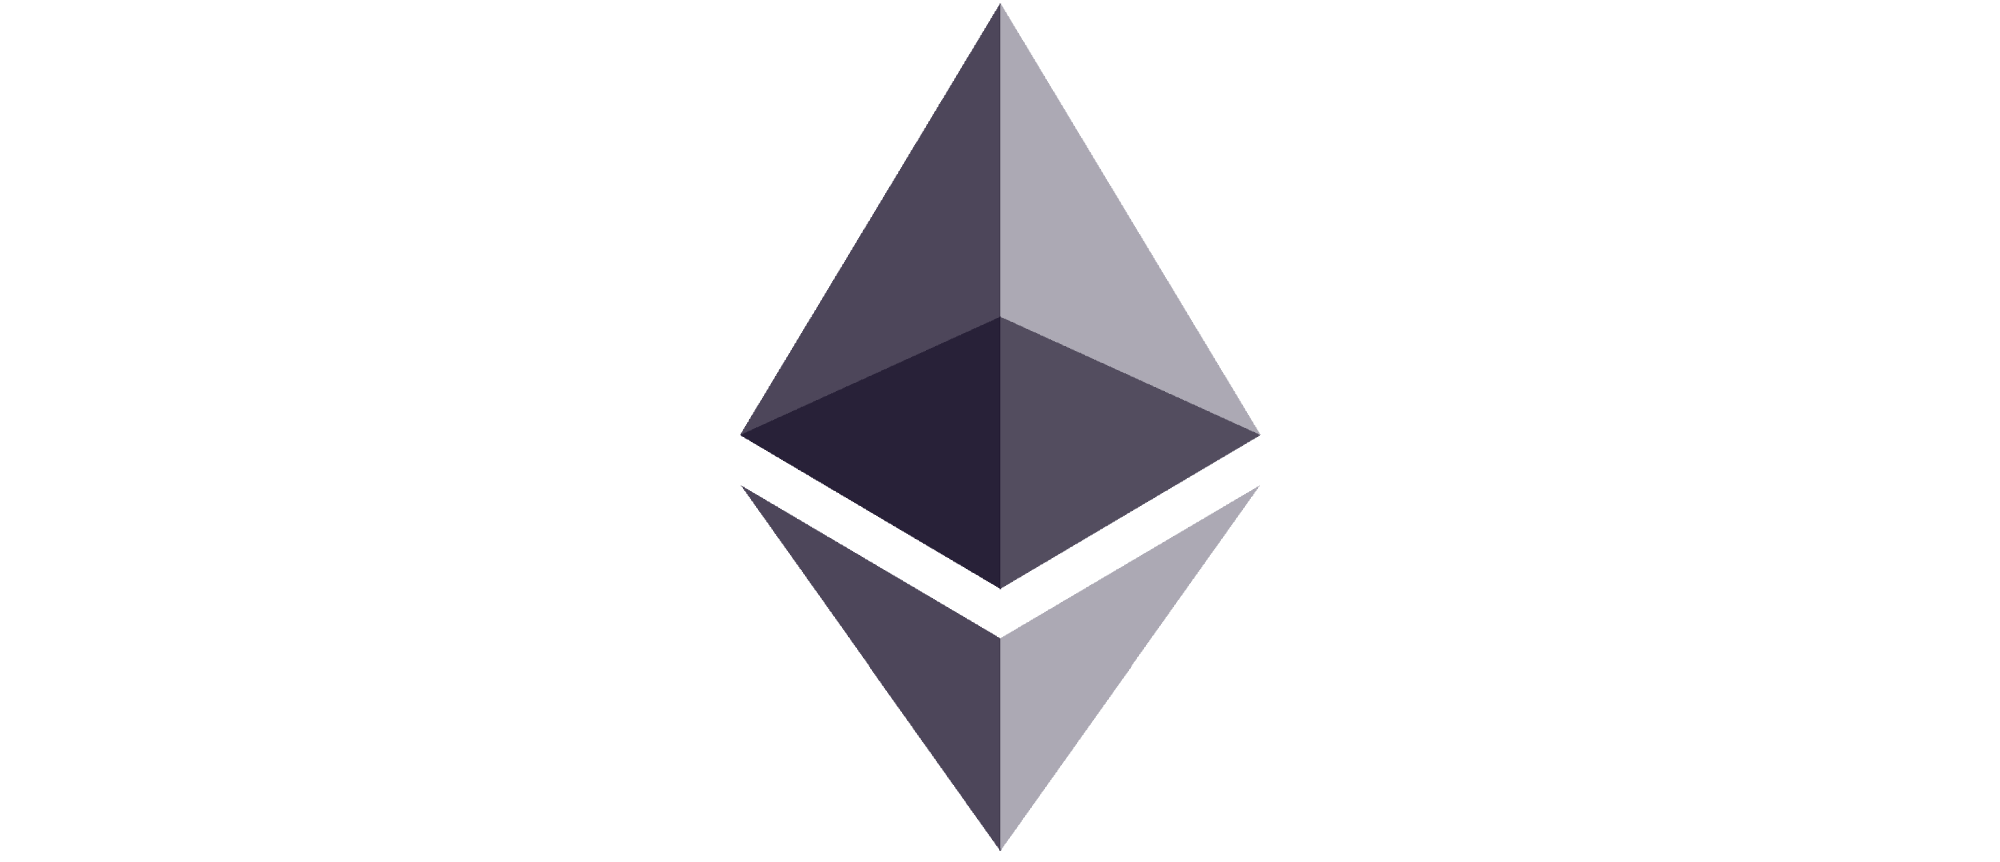
\includegraphics[width=\linewidth]{img/ethereum.png}
				\caption{Het Ethereum logo}
				\label{fig:ethereum}
			\end{figure}
			
			Ethereum is ontworpen met de volgende filosofie in gedachten (Ethereum Wiki)\footnote{zie https://github.com/ethereum/wiki/wiki/White-Paper\#ethereum}:
			\begin{itemize}
				\setlength\itemsep{1em}
				\item \textbf{Simpliciteit}: 
				Een van de hoofddoelen van Ethereum is om zo simpel mogelijk te zijn, zelfs als dit soms ten koste komt van data-opslag of tijdefficiëntie. Ethereum werd ontworpen met de bedoeling dat een gemiddelde programmeur, zonder een diepgaande kennis van cryptografie, er applicaties op zou kunnen implementeren. De bedoeling is dat de lage instapdrempel die de simpliciteit van Ethereum creëert er toe bijdraagt dat het ongekende potentieel van cryptocurrencies en blockchain technologie verder uitgebouwd wordt.
				\item \textbf{Universaliteit}: Ethereum doelt er op om Turingcompleet te zijn. Men wil  geen systeem aan bieden waar er gebruik kan worden gemaakt van bepaalde features, men wil een platform aan bieden waarop ontwikkelaars zelf iedere mogelijke toepassing kunnen implementeren aan de hand van smart-contracts en transacties.
				\item \textbf{Modulariteit}: 
				Een ander belangrijk aspect in het ontwerp van Etheruem is modulariteit. De bedoeling is dat de verschillende onderdelen waaruit Ethereum is opgebouwdt, zaken zoals Ethash, Patricia bomen en RLP, zo scheidbaar mogelijk worden gehouden. De verschillende bouwstenen van Ethereum worden als feature-complete bibliotheken gezien en kunnen ook buiten Ethereum gebruikt worden.
				\item \textbf{Agiliteit}: 
				Ethereum moet op een agile manier ontwikkelt worden. Men moet heel flexibel kunnen zijn op het vlak van aanpassingen. Hoewel men heel voorzichtig is wanneer het aankomt op modificaties bij high-level constructies, heeft Ethereum ook het doel om nieuw ontdekte mogelijkheden die verbetering brengen aan het systeem zo snel mogelijk te benutten.
				\item \textbf{Non-discriminatie en Non-censuur}: 
				Tot slot zou Ethereum niet mogen aansturen op een bepaalde vorm van gebruik. De regulerende mechanismen in het protocol moeten op zodanig wijze ontwikkelt zijn dat ze alleen schade zelf tegenhouden en niet specifieke ongewenste applicaties. Het voorbeeld van een oneindige lus wordt hier gegeven. Een applicatie die zo'n lus bevat is  ongewenst omdat ze middelen van het netwerk in beslag zal nemen en zo de verwerking van informatie zal vertragen. Toch wordt een degelijke applicatie niet verboden door Ethereum. Het regulerende mechanisme dat een transactiekost per computationele stap garandeert zorgt er immers voor dat een oneindige lus uitvoeren bijzonder nadelig wordt.
			\end{itemize}
	\subsection{Werking van Ethereum}
		De werking van het Ethereum-netwerk volgt op een hoog conceptueel niveau dezelfde lijnen als de eerder omschreven Bitcoin Blockchain~\autocite{Wood2017}. In dit segment wordt daarom vooral de foucs gelegd op de verschillen met Bitcoin. 
		
		In tegenstelling tot de (relatief) eenvoudige bitcoin-transacties, bevatten de blokken die door het Ethereum netwerk wordt opgeslagen iets wat men zou kunnen omschrijven als een toestandsmachine, bestaande uit een lijst van allerhande transacties. Waar de Bitcoin blockchain voornamelijk ontworpen is om fiscale transacties mogelijk te maken, is de Ethereum blockchain meer general-purpose~\autocite{McCorry2017}. Om misbruik en spamming van transacties tegen te gaan en spoedige verwerking te stimuleren is er aan iedere transactie een kleine kostprijs verbonden. Transactie en uitvoerings kosten worden \textit{gas} genoemd en betaald in ether, het cryptogeld van Ethereum. De naam gas is toepasselijk omdat men ether omschrijft als de brandstof waarop het Ethereum netwerk draait (Ethereum Wiki)\footnote{zie https://github.com/ethereum/wiki/wiki/White-Paper\#messages-and-transactions}.
		
		Binnen Ethereum is er sprake van twee soorten accounts: 
		\begin{itemize}
			\item Accounts van externe gebruikers, bestaande uit een publieke en private sleutel, dewelke een gebruiker in zijn bezit heeft.
			\item Contract accounts, smart-contract dewelke bestaan uit code die enkel wordt uitgevoerd bij interactie met gebruikers.
		\end{itemize}	
		Zowel gebruikers als smart-contracts kunnen ether bewaren ~\autocite{McCorry2017}. 
		
		Naast beide accounttypes zijn ook transacties van significant belang voor de werking van Ethereum. De Ethereum blockchain kan gezien worden als een geordende transactie-staat machine~\autocite{McCorry2017}. Net als bij Bitcoin zijn het  de transacties die  de core van het systeem vormen. Ethereum's transacties worden in een blockchain structuur opgeslagen, wat de volledige historiek van transacties oplevert, die  op haar beurt de huidige staat van het netwerk weergeeft.
		
		Een Ethereum-transactie bestaat uit de volgende velden (Ethereum Wiki):
		\begin{itemize}
			\item \textbf{From}: De ondertekening van het account dat de transactie autoriseert, dit kan alleen een gebruiker zijn.
			\item \textbf{To}: De ontvanger van de transactie, dit kan zowel een gebruiker als een contract zijn. 
			\item \textbf{Data}: Een optioneel veld. Hier  kan code meegegeven worden, ofwel voor de creatie van een smart contract, ofwel voor het uitvoeren van een smart contract.Er kan ook andere data worden meegegeven worden.
			\item \textbf{Gas Price}: Bedrag in ether dat de kost voorstelt die de verzender betaald per computationele stap.
			\item \textbf{Start Gas}: Het maximum aantal computationele stappen die mag worden uitgevoerd door de transactie.
			\item \textbf{Amount}: Bedrag in ether dat wordt overgemaakt van zender naar ontvanger.
		\end{itemize}	
		Transacties in Ethereum vinden plaats tussen twee gebruikers of tussen een gebruiker en een smart contract. Een transactie tussen een gebruiker en een smart contract kan één of meerdere nieuwe transacties vanuit het contract naar andere gebruikers doen ontstaan. Tenslotte kan een transactie van een gebruiker naar een smart contract ook transacties naar andere smart contracts triggeren, die dan op hun beurt hetzelfde doen en zo complexe kettingreactie creëren. De combinatie van mogelijke transacties en het potentieel dat smart contracts bieden zorgt voor een systeem waarop in theorie iedere toepassing mogelijk is~\autocite{Wood2017}. 
	\subsection{Conclusie}
		 Ethereum is een platform dat blockchain-technologie beschikbaar en toegankelijk maakt voor gewone ontwikkelaars. Een van Ethereums hoofddoelen is dan ook om multi-purpose te zijn: het is bedoelt als een platform waarop iedere mogelijke blockchain toepassing op geïmplementeerd kan worden. In deze sectie bespraken uitgebreid de filosofie waar Ethereum rond ontworpen is, in het algemeen kan men stellen dat de focus vooral ligt op de functionaliteit en gebruiksvriendelijkheid naar ontwikkelaars toe. Voorbeelden hiervan zijn de keuzes op het vlak van modulariteit en agiliteit. Men probeert duidelijk ook een omgeving te creëren waarin er zoveel mogelijk vrijheid is op vlak van het type van implementatie, geen enkele applicatie wordt geweerd op basis van haar functie. Alleen applicaties de voor schade aan het netwerk zelf zorgen worden niet toegelaten, dit om de werking van het volledige blockchain intact te houden. 
		
		\newpage
\section{Blockchain gebaseerd stemmen}
\label{sec:blockchain-gebaseerd-stemmen}
	\subsection*{Inleiding}
			In het derde een laatste deel van dit hoofdstuk wordt Blockchain gebaseerd stemmen besproken.  Als eerste wordt de noodzaak aangebracht, daarna worden bestaande implementaties besproken. De werking en achterliggende theorie worden als laatste besproken. Concreet bespreken we het Open Vote Network, een stemprotocol dat  aan de hand van smart contracts en Ethereum wordt geïmplementeerd. We bespreken dit protocol omdat het een van de weinige blockchain gebaseerde stemprotocollen is die volledig open source is. Er zijn ongetwijfeld veel andere manieren om een blockchain gebaseerd stemsysteem te realiseren,  hetgeen we hier bespreken is dus maar één voorbeeld, bedoeld ter illustratie.  In het vorige hoofdstuk bespraken zowel Ethereum als smart contracts reeds uitvoerig, in dit hoofdstuk zal de focus daarom meer op het cryptografische aspect liggen van het stemmen liggen. De werking van het stemprotocol wordt stap voor stap uitgelegd. De volledige natuur van de onderliggende cryptografie valt vaak buiten de scope van deze bachelorproef, bepaalde cryptografische technieken en wiskundige concepten worden daarom enkel vermeld en niet verder uitgewerkt. Tot slot wordt ook een selectie van bestaande implementaties besproken.
			Het concept blockchain gebaseerd stemmen bevind zich duidelijk nog in een vroeg stadium, men kan het zien als een onderdeel van wat \textcite{Swan2015} classificeert als blockchain 3.0 ofwel de blockchain implementaties van de toekomst.
	\subsection{Noodzaak}
			\subsubsection{Democratie en stemmen}
			Democratie wordt gedefinieerd als: ``een systeem waar bestuur van een natie door de volledige bevolking gebeurt, of op zijn minst door de in aanmerking komende leden er van''\footnote{ Definitie van democratie door Oxford Dictonairies, vertaalt uit het Engels. Verkregen op 1 Mei 2019 van https://en.oxforddictionaries.com/definition/democracy.}. In de meeste democratieën wordt het bestuur niet op een directe wijze door de bevolking uitgeoefend, maar via verkozen vertegenwoordigers. Om een democratie te laten functioneren moeten er dus processen zijn om vertegenwoordigers aan te duiden.  Aan de basis van elke succesvolle democratie ligt daarom de voorwaarde dat men kan stemmen op een wijze die toegankelijk, veilig en correct is.~\autocite{Osgood2016}. 
			
			Klassieke verkiezingen gebeuren aan de hand van een stem op papier: Men duidt de voorkeur aan op een stembiljet, vouwt het dicht en werp dit vervolgens in een `zwarte doos' waar alle stembiljetten ongeopend in blijven liggen tot ze geteld worden. Het tellen gebeurt handmatig, ambtenaren of burgers worden door een centraal stembureau opgeroepen om lokale stemmen te tellen. De resultaten worden vervolgens doorgeven aan hogere niveaus tot er uiteindelijk een volledig resultaat bekend is\footnote{ Omschrijving van hoe stemprocessen op papier doorgaans verlopen, lokale variaties zijn uiteraard mogelijk}.
			
			\subsubsection{Elektronisch stemmen}
			Hoewel de papieren stem al eeuwen gebruikt wordt zijn er toch een aantal problemen aan verbonden. In recente decennia heeft het zogenaamde elektronisch stemmen dan ook een enorme opkomst gekend. Ook in België, met name in het Vlaamse Gewest is dat het geval: in maar liefst de helft (157/300) van de Vlaamse gemeenten wordt vandaag gebruik gemaakt van stemcomputers (figuur \ref{fig:evote_vlaanderen}).
			
			\begin{figure}
				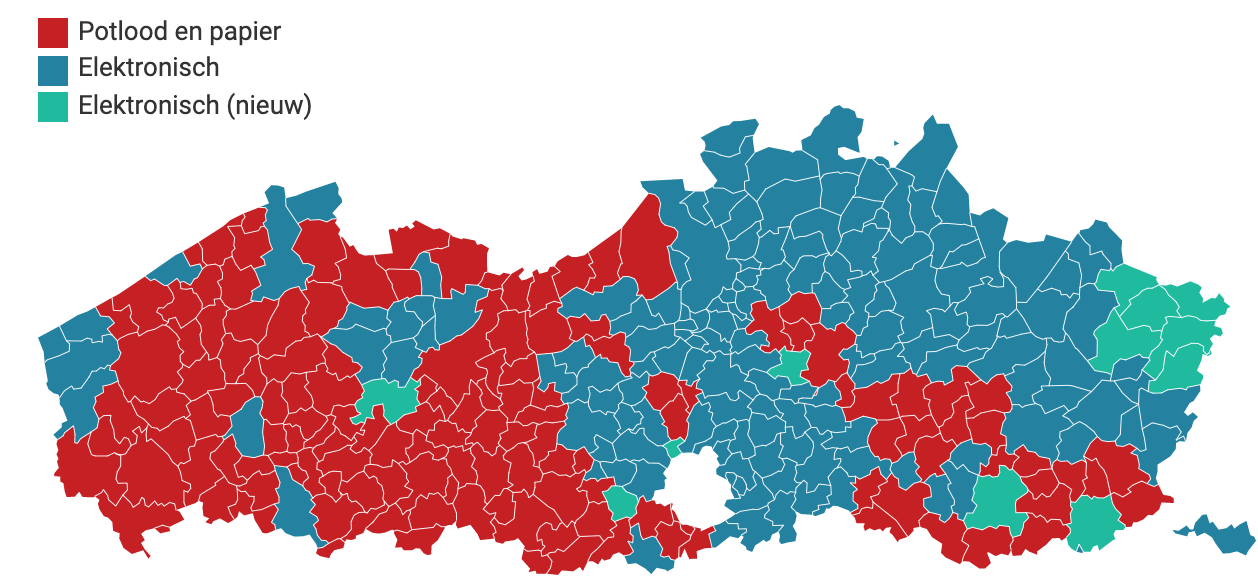
\includegraphics[width=\linewidth]{img/evote_vlaanderen.png}
				\caption{De helft van de Vlaamse gemeenten stemt digitaal (2018)}
				\label{fig:evote_vlaanderen}
			\end{figure}
			
			Volgens Smartmatic, leverancier van de stemcomputers in België en vele andere landen, biedt de elektronische stem een aantal aanzienlijke voordelen ten opzichte van de klassieke, papieren stem. Een van de voornaamste argumenten is dat de correctheid van de papieren stem in vraag kan worden gesteld gezien het proces bijzonder gevoelig is aan menselijke fouten, het zij opzettelijk of onopzettelijk. Een ander argument is dat de papieren stem veel minder \textit{toegankelijk} en \textit{efficiënt} is. Elektronisch stemmen daarentegen zou het stemproces voor vrijwel iedereen toegankelijk maken, ook personen met een lichamelijke of verstandelijke beperking zouden erdoor zelfstandig èn met behoud van het stemgeheim hun stem kunnen uitbrengen. Tenslotte is de elektronisch stem volgens Smartmatic ook efficiënter (en dus economisch voordeliger) dan de papieren variant. Elektronisch stemmen is namelijk veel sneller, het stelt grote landen in staat om de resultaten van hun verkiezingen in enkele uren te bereken, in de plaats van enkele weken.
			
			\subsubsection{Problemen met elektronisch stemmen}
			Hoewel de genoemde argumenten voor elektronisch stemmen grond hebben, zijn er ook argumenten tegen het elektronisch stemmen te voeren. Uit het onderzoek \cite{Norden2015} blijkt bijvoorbeeld dat een groot deel van de stemcomputers die worden gebruikt voor verkiezingen in de VS sterk verouderd zijn. Naar schatting gebruikte in 2015 maar liefst 43 van de 50 staten nog stemcomputers die op al minstens 10 jaar oud waren, in 14 van de staten zouden er zelfs machines zijn geweest die al meer dan 15 jaar oud waren. De leeftijd van stemcomputers zorgde volgens \cite{Norden2015} tijdens  congresverkiezingen van 2014 voor problemen gaande van vastlopende en uitvallende machines met als gevolg  lange wachtrijen, tot verloren en omgedraaide stemmen (op een andere kandidaat) met als gevolg verkeerde resultaten.
			
			Verouderde software zorgt er voor dat machines die gebruik maken van internet connecties bijzonder kwetsbaar zijn. De beveiligingen van zulke machines zijn niet meer adequaat volgens hedendaagse encryptie standaarden. Externe partijen kunnen in theorie zonder veel moeite toegang tot de zulke stemcomputers krijgen tijdens verkiezingen. Verouderde hardware zorgt er dan weer voor dat reparatie- en onderhoudskosten voor oude stemmachines bijzonder hoog zijn~\autocite{Norden2015}.
			
			Ook in België en Nederland krijgt elektronisch stemmen vaak de wind van voren. Tijdens de Belgische federale verkiezingen van 2014 bleek bijvoorbeeld dat er bij 57 stemcomputers een probleem had plaatsgevonden waardoor in totaal 2250 stemmen verloren gingen. In reactie daarop besliste Wallonië in 2015 voor een volledige terugkeer naar de papieren stem~\autocite{Maddens2018}.  In Nederland werden stemcomputers reeds in 1996 geïntroduceerd, maar ook hier zorgde toenemende problemen uiteindelijk in 2009 voor een terugkeer naar potlood en papier ~\autocite{Schellevis2018}.
			
			\subsubsection{Blockchain gebaseerd stemmen}
			Het is duidelijk dat er goede argumenten voor en tegen zowel papier als elektronisch stemmen kunnen gevoerd worden. Een blockchain gebaseerd stemsysteem zou volgens proponenten van de technologie een nieuwe manier kunnen vormen om elektronische stemmen te realiseren. Het zou veel van de huidige nadelen en problemen van elektronisch stemmen kunnen elimineren  en tegelijk ook de bestaande voordelen ten opzichte van stemmen op papier behouden. De gedistribueerde aard van blockchain zou er bovendien voor kunnen zorgen dat verkiezingen transparanter, veiliger en correcter dan ooit worden. 
			 
	\subsection{Bestaande Implementaties}
			\subsubsection{Concrete Toepassingen}
			Tot op heden zijn operationele toepassingen van blockchain stemsystemen nog relatief zeldzaam.  Er dient wel  een onderscheid gemaakt te worden tussen de verschillende soorten toepassingen. Men kan  blockchain technologie immers op diverse wijzen inzetten in de context van verkiezingen. In veel gevallen wordt een blockchain enkel ter ondersteuning van een groter stemsysteem gebruikt. Dit kan bijvoorbeeld zijn door blockchain als  een onveranderlijke opslagplaats te gebruiken voor de resultaten van een verkiezing. Een andere mogelijkheid is om blockchain technologie als verificatie tool te gebruiken. Er zijn echter ook implementaties die volledig blockchain gebaseerd zijn. Voor dit onderzoek zijn deze implementaties natuurlijk het interessantst ~\autocite{Kshetri2018}.
			
			In de volgende paragrafen worden 4 recente cases besproken waarin blockhain stemsystemen werden gebruikt ~\autocite{Kshetri2018}:
			\begin{enumerate}
				\item Parlements verkiezingen in Sierra Leone
				\item De jaarlijkse algemene vergadering van het Estse technologiebedrijf LVH Groep
				\item De gemeenschapsprojecten in Zuid-Koreaanse provincie Gyeonggi-do
				\item Het Active Citizen-programma van de stad Moskou
			\end{enumerate}
				
				\paragraph{Parlements verkiezingen in Sierra Leone}
				In maart 2018 werd in Sierra Leone blockchain technologie gebruikt om een kleine deelset van de resultaten van de nationale verkiezingen te controleren. Het systeem werd opgezet door het Zwitsers bedrijf Agora, dat aanwezig was als een internationale observator van de verkiezingen. Agora creëerde veel oproer door miscommunicaties de wereld in te sturen die  deden lijken dat de hele verkiezing op hun blockchain systeem was gebeurd. In feite deed Agora's implementatie enkel het tellen en bewaren van resultaten op basis van een blockchain. Bovendien werd slechts een fractie van de populatie geobserveerd, de manier waarop dit gebeurde was daarbovenop ook erg foutgevoelig. Men verzamelde, onafhankelijk van de verkiezingen, via bevraging het stemgedrag van ruim 400,000 kiezers. Tijdens dit verzamelen werd de data live aan een blockchain systeem gevoed. Het resultaat werd op gedistribueerde wijze berekend, ettelijke dagen voordat de klassieke telling afgerond was. De resultaten van Agora's telling kwam echter niet overeen met die van de overheid. Dit voorbeeld, hoewel niet bepaald  inspirerende op vlak van correctheid en fouttolerantie, is toch opmerkelijk omdat het wel aantoont hoe veel sneller en efficiënter blockchain systemen kunnen werken ten opzichte van klassieke manuele tellingen. ~\autocite{Kshetri2018}
				
				\paragraph{De jaarlijkse algemene vergadering van het Estse technologiebedrijf LVH Groep}
				Aandeelhouders van de Esthetische onderneming LVH Groep maken sinds 2015 gebruik van een kleinschalig online blockchain gebaseerd stemsysteem ~\autocite{Kshetri2018}. LVH Groep is een bankiers en financiële diensten bedrijf dat zich gespecialiseerd heeft in blockchain technologie, onder meer door een Bitcoin-wallet te ontwikkelen\footnote{ttps://www.coindesk.com/lhv-bank-backs-wallet-app-built-on-bitcoins-blockchain}. Doordat LVH groep een internationale onderneming is met kantoren in verscheidene landen, was het enorm kostlijk en tijdsrovend om op jaarlijkse basis alle aandeelhouders op een plaats te verzamelen voor een algemene vergadering. Er was  nood aan een veilig systeem om beslissingen over het internet te kunnen maken. Hiertoe werd in samenwerking met onder andere de bedrijven NASDAQ en Chain een systeem geïmplementeerd op de Bitcoin blockchain dat werkt op basis van smart contracts. Verificatie van de kiezers wordt gedaan door gebruik te maken van het bestaande digitale identiteitssysteem in Estland \footnote{http://francescoolcelli.blogspot.com/2017/01/is-blockchain-answer-to-e-voting-nasdaq.html|}. Bijzonder aan deze implementatie was dat ze aantoonde dat ook zonder directe ondersteuning van het platform, er zeer veilige en betrouwbare implementaties kunnen gemaakt worden op blockchain. ~\autocite{Kshetri2018}
				
				\paragraph{De gemeenschapsprojecten in Zuid-Koreaanse provincie Gyeonggi-do}
				In maart 2017 maakte het provinciebestuur van de Zuid-Koreaanse provincie Gyeonggi-do gebruik van een blockchain implementatie om burgers via directe verkiezingen te laten  bepalen welke gemeenschapsprojecten gefinancierd dienden te worden. Burgers konden zelf voorstellen doen en op suggesties van medeburgers stemmen. Het overkoepelende Ddabok Community Support Project zag maar liefst 9000 inwoners participeren. In totaal werden rond de 500  projecten geselecteerd voor subsidies. Het bijzondere aan deze implementatie was dat hoewel, georganiseerd vanuit de overheid, er geen enkele centrale autoriteit in het stemproces was betrokken. Het hele systeem werd ontwikkeld door Blocko, de grootste Zuid Koreaanse blockchain firma. ~\autocite{Kshetri2018}
				
				\paragraph{Het Active Citizen-programma van de stad Moskou}
				De stad Moskou kent sinds 2014 een programma genaamd Active Citizen waarbij haar inwoners via zowel mobiele als online applicaties (zie figuur \ref{fig:active_citizen}) kunnen stemmen over allerhande maatregelen, gaande van de naam voor een nieuwe metro-trein tot de kleuren van zetels in een nieuw sport-stadion. Het Active Citizen-programma telt meer dan 2 miljoen geregistreerde kiezers, er werden tot heden al meer dan 92 miljoen stemmen op uitgebracht. De laatste jaren is er echter steeds minder vertrouwen in de stad wanneer het op het tellen van de stemmen aankomt. Om de inwoners gerust te stellen en vertrouwen terug te winnen werd  daarom in 2017 een private versie van de Ethereum blockchain aan de architectuur van het project toegevoegd. ~\autocite{Kshetri2018}
				
				\begin{figure}
					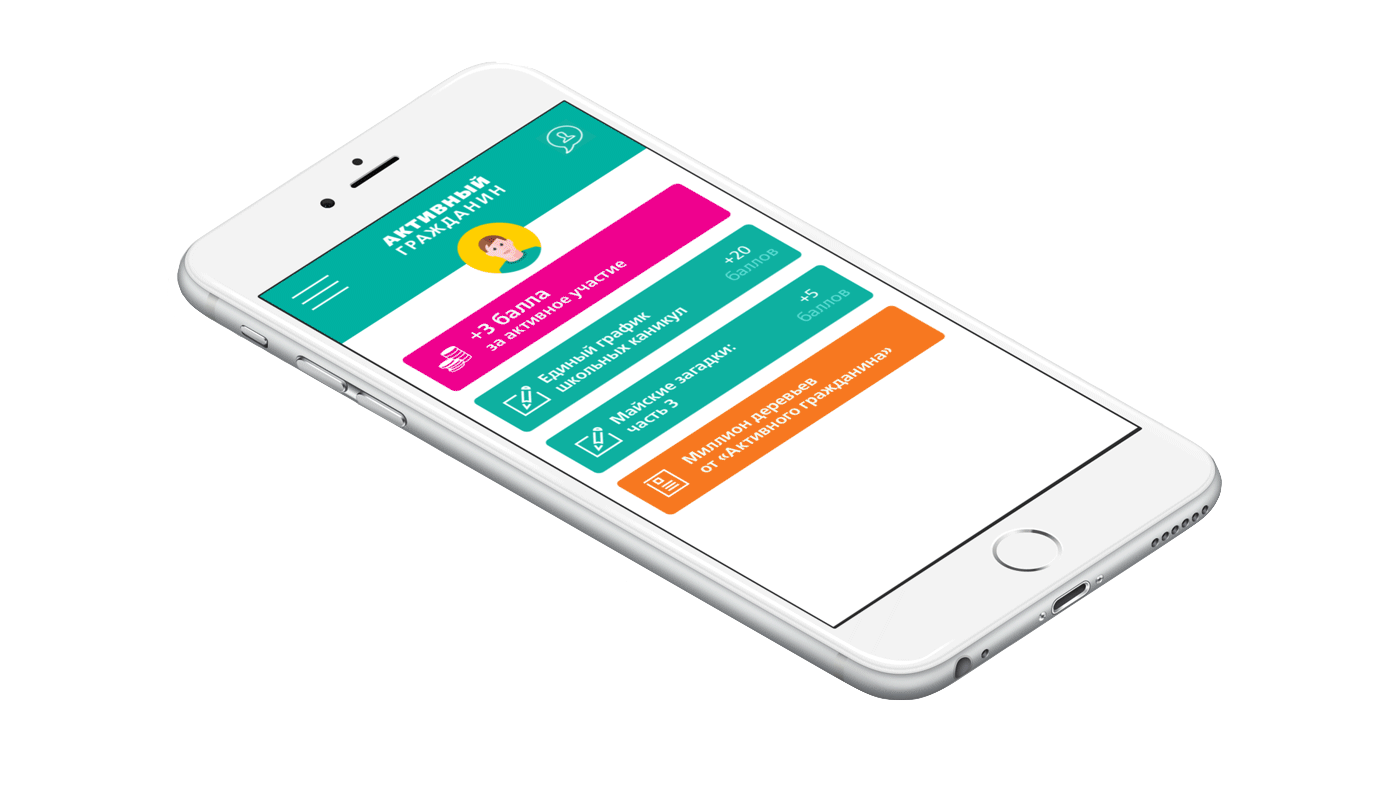
\includegraphics[width=\linewidth]{img/active_citizen.png}
					\caption{Het Active Citizen programma via een mobiele applicatie}
					\label{fig:active_citizen}
				\end{figure}
				
				Zoals vermeld gaat het om een Ethereum implementatie. Er wordt gewerkt aan de hand van smart contracts om de stemmen te registreren. Alle stemmen komen terecht in een  blockchain, het resultaat van alle verkiezingen is publiek beschikbaar. Ook de broncode voor de implementatie werd publiek gemaakt op GitHub.
				
				De populairste onderwerpen zagen tussen de 137.000 tot 220.000 participanten. Tijdens testen was de  Ethereum implementatie  instaat om tot 1000 transacties per minuut te verwerken. Het is niet duidelijk of de implementatie overweg zou kunnen met  grotere volumes van kiezers. De schaalbaarheid is in deze context wel noodzakelijk, men wil een systeem bekomen dat toegankelijk is voor iedere bewoner en Moskou telt immers een 12 miljoen inwoners. De kans is groot dat het huidige systeem overrompelt zou raken en compleet zou verstoppen moesten miljoenen kiezers gelijktijdig hun stem uitbrengen.
				
				Op het vlak van security is schaalbaarheid dan weer geen probleem. De stads administratie liet het systeem testen door PwC, een internationaal accountants- en belastingadviseursbedrijf. De bevindingen van PwC waren dat er geen reden tot bezorgdheid is voor de veiligheid bij  300.000 of meer kiezers. 
				
				Al bij al levert dit voorbeeld toch een sterke case op voor de blockchain gebaseerd stemmen op grote schaal. Het toont aan dat men met voldoende middelen blockchain stemprotocollen kan ontwikkelen die qua scope de klassieke board-room voting systemen uit de literatuur vele malen overtreffen. 
			\subsubsection{Online Diensten}
				\paragraph{The Blockchain Voting Machine }
					Een van de grootste argumenten tegen blockchain gebaseerd stemmen is dat het een verhoogd risico met zich meebrengt, de bestaat  dat de nodes overgenomen worden of al overgenomen zijn. Voor een systeem dat werkt over het internet zou het gevaar van een nog grotere orde zijn. The Blockchain Voting Machine is hier heel simpele antwoord op: men stelt voor om te werken met elektronische stemmachines zoals die vandaag al bestaan,   de machines zijn echter niet aan het internet verbonden alleen aan een privaat blockchain netwerk. 
				\paragraph{FollowMyVote}
					Het online stemplatform FollowMyVote hanteert de tegenovergestelde redenatie van The Blockchain Voting Machine. Het uitgangspunt van dit opensource platform is net dat blockchain de ideale technologie is om verkiezingen niet alleen elektronisch maar ook online te maken. Online-verkiezingen zijn nodig volgens FollowMyVote omdat het de kosten van verkiezingen enorm kan onderdrukken en de opkomst van kiezers vele malen groter kan maken.  Zwakkere groepen zoals bejaarden of invaliden, maar ook mensen in het buitenland kunnen nu  meestemmen.  Op het vlak van identificatie stelt men voor om te werken met behulp van webcams en door de overheid uitgegeven identiteitsbewijzen. Het resultaat van verkiezingen wordt in de blockchain opgeslagen, de resultaten zijn publiek verifieerbaar. FollowMyVote stelt ook een reeks andere functionaliteiten waaronder: real-time verkiezingen volgen en een stem die binnen de verkiezingstermijn aangepast kan worden. 
				\paragraph{TIVI}
					TIVI hanteert heeft ongeveer dezelfde motivatie als FollowMyVote, maar op vlak van identificatie neemt men het hier nog een stap verder. Men stelt voor om stemmen mogelijk te maken vanaf eender welk platform, zij het laptop, mobiel of tablet. Verificatie kan volledig via gezichtsherkenning gebeuren volgens TIVI, zodat men zich kan identificeren door een selfie te nemen.
				\paragraph{Agora}
					Agora is een Zwitsers bedrijf dat een platform ontwikkeld heeft voor blockchain gebaseerde stemsystemen. Agora heeft een eigen custom blockchain infrastructuur opgezet en bouwt middel tot grote verkiezingstoepassing op maat voor haar klanten. Agora geldt momenteel als een van de grootste spelers in de sector.
					
	\subsection{Cryptografie en Stemprotocollen}
		\subsubsection{Verschillende Protocollen}
		\textcite{Kiayias2002} stelt voor om stemprotocollen self-tallying te maken. Self-tallying ofwel zelf-tellend wordt hier gedefinieerd als volgt: iedere kiezer moet na het einde van een stemming zelf de stemmen kunnen tellen. Zelf-tellende stem-protocollen nemen de verantwoordelijk voor het tellen van stemmen weg van centrale autoriteiten en veranderen het in een open procedure, die iedere deelnemer of derde partij kan uitvoeren. De centrale tellingsautoriteit is dan niet meer nodig, iedereen kan resultaat van de stemming onafhankelijk bekomen. Men definieert ook twee andere eigenschappen waaraan een elektronisch stem-protocol moet voldoen.  Perfect Ballot Secrecy ofwel volledige stembescherming, wordt gedefinieerd als een eigenschap die de verzekering brengt dat de privacy van de stemmer enkel en alleen kan ondermijnd worden als alle andere stemmers tot dit doeleinde collaboreren. Dispute-freeness ofwel geschil-vrijheid, wordt dan weer gedefinieerd als een eigenschap die garandeert dat dat er geen twijfel kan zijn over de authenticiteit van de stemming. Deze eigenschap bestaat eruit dat iedere participant van de stemming, na afloop het correcte verloop van de procedure kan verifiëren voor zichzelf.
			
		Volgens \textcite{McCorry2017}  hebben deze zelf-tellende protocols zwaktepunten op het vlak van eerlijkheid. Ze laten toe dat de alle personen die gestemd hebben op een bepaald tijdstip, zouden kunnen collaboreren om de tussen-resultaten te berekenen voor datzelfde tijdstip. Verder kan de laatste persoon die zijn of haar stem moet uitbrengen het resultaat van de stemming berekenen voor hij of zij effectief gestemd heeft. Dit leidt volgens \textcite{McCorry2017} tot adaptive en abortive issues.  \textcite{McCorry2017} spreekt van een adaptive issue waar de stemkeuze van de laatste participant mogelijks beïnvloed kan worden door het zien van de stemresultaten voor zelf te stemmen. Er is ook sprake van een abortive issue volgens \textcite{McCorry2017} omdat iedere participant de macht heeft om de hele stemming te annuleren. Een enkele participant kan zich immers volledig kunnen onthouden van het stemmen en zo alle andere stemmers verhinderen het resultaat te berekenen. 
			
		\textcite{Kiayias2002} stelt dat het bovenstaande probleem makkelijk te corrigeren valt door middel van een extra stemronde. \textcite{McCorry2017} stelt echter dat daarvoor de volledige coöperatie van alle participanten nodig is, en dat deze niet meer gegarandeerd is op dit punt. Ook wordt er voorgesteld om de laatste stem steeds een lege stem van de organisator te laten zijn, maar ook hiertegen verzet \textcite{McCorry2017} zich, men stelt dat dit in essentie een terugkeer is naar een systeem met centrale autoriteit.  \textcite{McCorry2017} stelt een protocol voor, op basis van het werk van Kiayias and Yung en Groth maar combineert als eerste het concept van self-tallying met een blockchain implementatie. Het resulteren protocol noemt men het \textit{Open Vote Network Protocol} (OVNP).
		
		 \textcite{McCorry2017} maakt gebruik van Ethereum als ontwikkelplatform voor het OVNP. In sectie \ref{sec:ethereum-en-smart-contracts} bespraken we de verschillende voordelen die dit platform biedt reeds uitgebreid. Ook \textcite{Dagher2018} stelt met BroncoVote een stemsysteem voor dat werkt via Ethereum. BroncoVote is blockchain stemsysteem dat gebaseerd is op andere cryptografische methodes dan OVNP en bijgevolg sterk verschilt met protcollen van \textcite{Kiayias2002} en \textcite{McCorry2017}. 
	
	\subsection{Het Open Vote Network Protocol}
		\subsubsection*{Overzicht }
			Het Open Vote Network Protocol is een gedecentraliseerd protocol, ontworpen op basis van het self-tallying principe. De focus ligt hier op de bescherming van privacy en de robuustheid, niet op de schaalbaarheid. Self-tallying gebeurt immers niet op een wijze die bijzonder schaalbaar is. Het  Open Vote Network protocol ondersteund bijgevolg enkel kleine verkiezingen met tientallen participanten, zaken zoals nationale verkiezingen zijn momenteel  zo goed als onmogelijk. Om eenvoud te bewaren wordt er gewerkt met het simpelste verkiezingspatroon dat mogelijk is, deelnemers hebben de keuze tussen twee opties, bijvoorbeeld een ja/nee vraag.  \textcite{McCorry2017} verwijst naar het onderzoek van \textcite{Hao2010} voor zogenaamde multi-way verkiezingen ofwel verkiezingen met meerdere keuze-opties. 
			
			Het stemmen in dit protocol gebeurt in twee fasen, in de eerste fase laten alle kiezers zich registreren, in de tweede fase wordt de effectieve stem uitgebracht. Na afloop van de tweede fase kunnen de stemmen geteld worden.  De self-tallying eigenschap stelt iedere stakeholder die het protocol uitvoert ertoe instaat om zelf de stemmen te tellen. Merk op dat iedereen dit facet van het protocol kan uitvoeren, niet enkel de geregistreerde stemmers.
			 
			Het gedecentraliseerde karakter van dit protocol maakt het uiterst geschikt om op een blockchain te implementeren. \textcite{McCorry2017} is een van de eersten in de literatuur die deze stap maakt. De reden dat men specifiek voor de Ethereum blockchain kiest, wordt gemotiveerd als volgt.
			
			Andere blockhains zoals Bitcoin zouden ook kunnen worden gebruikt als publieke opslagplaats van verkiezingen, maar het verschil is dat het protocol niet op de blockchain kan opgeslagen worden, het moet extern dan opgeslagen en gehandhaafd worden door de kiezers. \textcite{McCorry2017} stelt dat men via Ethereum gebruik kan maken van een smart-contract om  het protocol af te dwingen, Ethereum kan daarnaast niet alleen als opslag fungeren maar ook als geverifieerd netwerk waarover de participanten communiceren.
		\subsubsection*{Fase 0: Setup }
			Het OVN-Protocol start vanuit een zogenaamde \textit{election administator}, deze organisator van de verkiezingen initialiseert het protocol door de een verkiezing aan te maken en de in aanmerking komende kiezers in te stellen, dit gebeurt door de kiezers aan de white-list van het smart-contract toe te voegen. De kiezers worden in dit stadium enkel geïdentificeerd aan de hand van hun Ethereum account. De organisator is meestal degene die  Ethereum verwittigt om over te schakelen op de eerste fase.
		\subsubsection*{Fase 1: Registratie }
			De administrator stelt het onderwerp van de verkiezing in, als ook de beschikbare opties waarvoor gestemd kan worden. Vervolgens wordt Ethereum opnieuw verwittigd, ditmaal om over te gaan naar de registratie van de participanten. Om te registreren voor de verkiezing moeten alle stemmers vooraf een stemsleutel berekenen. Deze sleutel zal worden gebruikt als identificatie van de kiezers. Het berekenen  van de stemsleutel en het verdere verloop (samengevat in figuur \ref{fig:ovnp}) gaat als volgt: 
			
			Alle \textbf{\textit{n}} kiezers moeten het eens zijn over het paar \textbf{\textit{(G,g)}} waarbij \textbf{\textit{G}} een eindige cyclische groep van hoofdorde \textbf{\textit{q}} voorstelt waar het Diffie-Hellman (DDH) probleem niet van toepassing op is, en \textbf{\textit{g}} een generator in \textbf{\textit{G}}. De lijst van in aanmerking komende kiezers, hier ook participanten \textbf{\textit{(P$_{1}$, P$_{2}$, … , P${n}$)}} genoemd, wordt vastgelegd. Elke participant \textbf{\textit{P$_{i}$}} kiest een unieke random waarde  
			
			\textbf{\textit{$x_{i} \in^{R} Z_{q}$}}.
			
			 De waarde \textbf{\textit{x$_{i}$}} wordt gebruikt als private stemsleutel. Iedere kiezer vormt zijn of haar publieke stemsleutel door \textbf{\textit{g$^{x_{i}}$}} te berekenen. Gezien \textbf{\textit{g}} een generator is van \textbf{\textit{G}}, valt niet te achterhalen aan de hand van \textbf{\textit{g$^{x_{i}}$}} wat de eigenlijke waarde van \textbf{\textit{x$_{i}$}} is. Het Ethereum netwerk heeft met andere woorden geen kennis van \textbf{\textit{x$_{i}$}}. Om de participant \textbf{\textit{P$_{i}$}} te kunnen identificeren in het netwerk volstaat de publieke sleutel echter niet, er is ook een bewijs van de private sleutel \textbf{\textit{x$_{i}$}} nodig. Tot dat doeleinde wordt een Zero Knowledge Proof gebruikt. Met \textbf{\textit{ZKP(x$_{i}$)}} levert de participant \textbf{\textit{P$_{i}$}}  het bewijs aan het netwerk dat de \textbf{\textit{x$_{i}$}}  in \textbf{\textit{g$^{x_{i}}$}} gekend is door \textbf{\textit{P$_{i}$}}. Zonder de waarde voor \textbf{\textit{x$_{i}$}}  effectief bekend te maken, wordt er zo bewezen dat \textbf{\textit{P$_{i}$}} de eigenaar van de publieke sleutel \textbf{\textit{g$^{x_{i}}$}} is.
			
			Registratie gebeurt door iedere kiezer \textbf{\textit{P$_{i}$}} te laten broadcasten naar het netwerk. De broadcast bestaat uit \textbf{\textit{g$^{x_{i}}$}}  en \textbf{\textit{ZKP(x$_{i}$)}}. Daarnaast wordt er ook een constante waarde in ether uit de portefeuille van de kiezer aan de broadcast toegevoegd. Het gaat hier om de som van de transactie kosten en een waarborg die de kiezer terugkrijgt. De waarborg instellen gebeurt omdat blockchain filosofie dicteert dat het verbinden aan een potentiele kost participanten zal stimuleren om oprecht te handelen, in dit geval geeft men de waarborg terug van zodra ze hun stem uitbrengen. 
			
			Nadat een kiezer \textbf{\textit{P$_{i}$}}  gebroadcast heeft naar Ethereum zal het netwerk zijn broadcast verwerken. Het bewijs in de vorm van de \textbf{\textit{ZKP(x$_{i}$)}} wordt gecontroleerd, de waarborg wordt opgeslagen en tot slot wordt de  stemsleutel \textbf{\textit{g$^{x_{i}}$}} gebruikt om een nieuwe sleutel te berekenen waarmee de kiezer \textbf{\textit{P$_{i}$}} een stem zal kunnen uitbrengen over het ingestelde onderwerp. Deze nieuwe sleutel noemt men de gereconstrueerde sleutel \textbf{\textit{g$^{y_{i}}$}}, ofwel \textbf{\textit{Y$_{i}$}} en wordt berekend als volgt: 
			\begin{ceqn}
				\begin{align}
					Y_{i} = \prod_{j=1}^{i-1}g^{x_{j}}  / \prod_{j=i+1}^{n}g^{x_{j}} \label{formula1}\
				\end{align}
			\end{ceqn}
			
			\eqref{formula1} \textit{Om de gereconstrueerde sleutel g$^{y_{i}}$ te berekenen van kiezer \textbf{P$_{i}$} worden de publieke stemsleutels van alle andere kiezers \textbf{P$_{j}$} gebruikt. Het product van de publieke sleutels van al de andere kiezers \textbf{P$_{j}$} waar j < i wordt gedeeld door het product van alle publieke sleutels van al de andere kiezers waar \textbf{P$_{j}$} waar  j > i.}
			
		\subsubsection*{Fase 2: Stemmen}
			Eenmaal het netwerk signaal ontvangt dat er gestemd kan worden, kunnen de kiezers een beslissing maken en vervolgens hun stem te broadcasten. Deze broadcast bestaat uit twee zaken: de geëncrypteerde stem en een nieuwe Zero Knowledge Proof, die bewijst dat de stem ofwel 0 of 1 is. De encryptie die gebruikt wordt voor de stem vormt het cryptografische hart van dit protocol. 
			
			De stem wordt geëncrypteerd volgens het Elgamal-cryptosysteem en wordt in de vorm  \textbf{\textit{g$^{x_{i}y_{i}}$g$^{v_{i}}$}} aan het netwerk doorgegeven,  waarbij  \textbf{\textit{g$^{x_{i}y_{i}}$}} het product is van de publieke stemsleutel en de gereconstrueerde sleutel, \textbf{\textit{v$_{i}$}} de eigenlijke stem is in de vorm van een 1 of een 0 en \textbf{\textit{g$^{v_{i}}$}} de factor waarmee het product van de sleutels vermenigvuldigt wordt, zijnde ofwel g ofwel 1. 
			
			Eenmaal \textbf{\textit{P$_{i}$}} de stem broadcast wordt aan de hand van de \textbf{\textit{ZKP(v$_{i}$)}} geverifieerd of de stem in een correct formaat is (0 of 1), is dit het geval dan wordt de Elgamal-geëncrypteerde stem opgeslagen in de Ethereum blockchain en wordt de waarborg aan \textbf{\textit{P$_{i}$}} geretourneerd.
			
			Wanneer alle n stemmen ontvangen en geverifieerd zijn krijgt iedereen er toegang toe. De identiteit van de kiezers noch de betekenis is door de encryptie niet meer af te leiden uit een particuliere stem. Alleen het resultaat kan nog bekomen worden uit de nu persistente geëncrypteerde stemmen.
			
			Het resultaat van de verkiezing bekomt men door het product van alle geëncrypteerde stemmen te nemen \eqref{formula2}: 	
			\begin{ceqn}
				\begin{align}
				\prod_{i=1}^{n}g^{x_{i}y_{i}}g^{v_{i}} \label{formula2}\
				\end{align}
			\end{ceqn}	
			De aard van de encryptie is van zodanig dat alle random factoren geëlimineerd worden \eqref{formula3}, zodat :	
			\begin{ceqn}
				\begin{align}
				\prod_{i=1}^{n}g^{x_{i}y_{i}} = 1 \label{formula3}\
				\end{align}
			\end{ceqn}
			Dit resulteert in:
			\begin{ceqn}
				\begin{align}
				g^{\sum_{i=1}^{n}v_{i}} \label{formula4}\
				\end{align}
			\end{ceqn}
			Waarbij \textbf{\textit{$\sum_{i=1}^{n}v_{i}$}} in \eqref{formula4}, het aantal stemmen voor waarde 1 representeert. Het aantal waar-stemmen kan echter niet rechtstreeks worden afgeleid, \textbf{\textit{g}}  wegwerken impliceert een discreet logaritme. Gezien de rechterhelft van de vergelijking bekend is en \textbf{\textit{i}} gelimiteerd is tot het aantal participanten \textbf{\textit{n}}, is het vrij zeker dat het hier om een kleine waarde gaat. Deze waarde kan gemakkelijk gevonden worden door middel van \textit{brute-force} zoeken. Eenmaal het aantal ja-stemmen gevonden is, wordt het vinden van de nee-stemmen triviaal.
			
			Merk op dat het noodzakelijk is bij self-tallying stemprotocollen dat iedere kiezer die in fase 1 een stemsleutel broadcast ook een geëncrypteerde stem uitstuurt in fase 2. Anders kunnen de resultaten van de stemming niet berekend worden. Er is hier dus nog steeds sprake van een \textit{abortive issue}.
			
			Ook is er het feit dat bij self-tallying stemprotocollen de allerlaatste kiezer mogelijks de stemmen kan tellen alvorens zelf te kiezen. Door een 0-stem te simuleren, kan deze kiezer het resultaat van de verkiezingen berekenen voordat alle anderen dit kunnen. De kiezer kan dus potentieel zijn of haar stem nog veranderen op basis van het voorlopige resultaat van de verkiezing. In de meeste gevallen is dit natuurlijk geen wenselijke situatie. De oplossingen die voor dit probleem in de literatuur worden voorgesteld zijn echter ook sub-optimaal volgens \textcite{McCorry2017}. 
			
			\textcite{McCorry2017} stelt voor om een fase toe te voegen tussen fases 1 en 2. In deze fase wordt de stem van de kiezer opgeslagen voor bekendmaking aan het netwerk, eenmaal opgeslagen kan de stem niet meer veranderen. De volgende fase bestaat er dan uit dat de stem bekent wordt gemaakt aan het netwerk. 

			\begin{figure}
				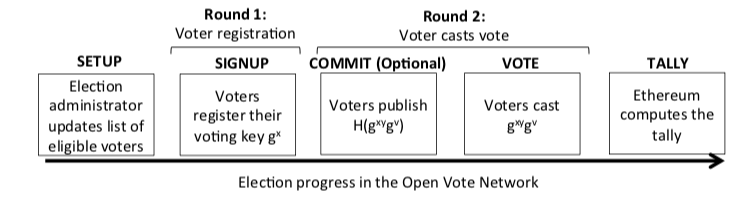
\includegraphics[width=\linewidth]{img/ovnp.png}
				\caption{Het Open Vote Network Protocol samengevat}
				\label{fig:ovnp}
			\end{figure} 
	
	\newpage
	\subsection{Privacy en transparantie}
		Typische elektronisch stem-protocollen beschermen de privacy van kiezers door gebruik te maken van een centrale autoriteit, om veiligheidsredenen is de autoriteit vaak verdeelt over verschillende tellings-autoriteiten. Een voorbeeld hiervan vinden we terug bij het stemsysteem van Helios\footnote{https://github.com/benadida/helios-server}. Elektronische stemmen worden hier door meerdere tellings-autoriteiten behandeld, in combinatie met cryptografie reduceert men het risico op aantasting van de gebruikers privacy aanzienlijk ~\autocite{Adida2008}. 
	
		Los van dit gegeven echter, staat het feit dat een dergelijk systeem gebaseerd op het vertrouwen van de stemmers. De mogelijkheid bestaat nog steeds dat alle tellingsautoriteiten van kwade wil zijn of dat ze simpelweg overrompeld worden door aanvallers. In zo’n situatie kan de privacy van de gebruikers alsnog geschaad zijn~\autocite{McCorry2017}.
		
		In essentie gaat het hier om een probleem op het vlak van transparantie, de gebruiker van het systeem heeft immers weinig tot geen middelen om zichzelf er van te verzekeren dat het hele proces correct verloopt~\autocite{McCorry2017}. 
		
		We bespraken verschillende manieren waarop blockchain technologie kan aangewend worden in elektronische stemsystemen. De verschillende wijzes die we bespraken kennen enkele noemenswaardige verschillen op het vlak van privacy. Het Open Vote Network dat voorgesteld wordt door \textcite{McCorry2017} vormt een van de meest robuuste structuren die de privacy van gebruikers garanderen. Volledige anonimiteit, zoals men heeft wanneer men een papieren stem in de stembus werpt, is niet mogelijk op blockchain, maar op basis van cryptografie slaagt \textcite{McCorry2017} er wel in om het vinden van andermans identiteit praktisch onmogelijk te maken. Merk op dat  de term identiteit hier niet persoonlijke gegevens van de gebruiker betekent, wel het Ethereum account van de gebruiker.
		
		Ook  de andere systemen die we bespraken, Agora, FollowMyVote, enz. lijken op het eerste zicht relatief goed te scoren op het vlak van privacy. Toch is er bij veel van de besproken voorbeelden een fundamenteel probleem op het vlak van centralisatie, aldus \textcite{McCorry2017}. De meeste voorgestelde oplossingen zijn nog steeds, in variërende mate, afhankelijk van een centrale autoriteit. Men zou het argument kunnen voeren dat bijvoorbeeld een bedrijf zoals FollowMyVote, hoewel hun hele stemproces op de blockchain gebeurd, op een bepaalde manier zelf een centrale autoriteit wordt wanneer men van hun diensten wil gebruik maken. Blockchain gebaseerde stemsystemen waarvan de codebasis  niet open source is, vergen daarboven op een bepaalde manier ook weer het vertrouwen van de gebruiker. Wanneer stemsystemen ook toegang krijgen tot gevoelige informatie zoals elektronische identiteitsgegevens of zelfs biometrische-data voor gezichtsherkenning, zoals het bedrijf TIVI voorstelt, dan speelt dit vertrouwen een rol die zodanig cruciaal is dat er eigenlijk sprake is van een centrale autoriteit.
	\subsection{Fouttolerantie, Veiligheid en Correctheid}
	
	Naast privacy en transparantie zijn ook fouttolerantie, veiligheid en correctheid van centraal belang in de context van stemprotocollen. Deze drie zaken zijn inherent aan elkaar verbonden, er is zelfs sprake van zekere grote overlapping. We definiëren kort de bovenstaande termen voor we bekijken hoe ze van toepassing zijn op blockchain-gebaseerde stemsystemen. \textit{Fouttolerantie} gaat in de eerste plaats over de robuustheid  van het systeem, het is de mate waarin het systeem bestendig is tegen allerhande fouten die zich kunnen voordoen. Een belangrijke distinctie is dat we het hier enkel over onopzettelijk fouten hebben. De mate waarin opzettelijk fouten en andere malafide acties een impact hebben op het systeem wordt gedefinieerd als de \textit{veiligheid}. Tenslotte definiëren we \textit{correctheid} als de mate waarin het berekende resultaat overeenkomt met de werkelijkheid en dit onder invloed van factoren zoals fouttolerantie en veiligheid.
	
	Op het vlak van fouttolerantie zijn er een paar inherente problemen met het OVN-protocol dat \textcite{McCorry2017} voorstelt. De voornaamste problemen zijn zogenaamde \textit{abortive issues} die te maken hebben met het missen van deadlines. Zoals vermeld wordt er in het OVN gewerkt met verschilleden fases, alle kiezers worden steeds veronderstelt om binnen deze fases bepaalde acties te ondernemen. Een kiezer die per ongeluk zo'n een deadline mist, bijvoorbeeld door het uitvallen van de netwerk-connectie, verliest niet alleen zijn voorafbetaalde waarborg, maar breekt ook de volledige verkiezing. De cryptografie van het systeem vereist immers dat iedere geregistreerde kiezer een stem uitbrengt, alvorens de resultaten kunnen berekent worden. Ook op het vlak van veiligheid vormt dit een probleem, het betekent dat voor de prijs van de waarborg, iedere participant de verkiezing kan boycotten. Tenslotte zal dit zich ook laten gelden op het vlak van schaalbaarheid en scope. 
	
	De andere kant van de medaille is hier dat het OVN-protocol wel zeer goed scoort op het vlak correctheid, het is moeilijk om het resultaat op frauduleuze wijze te beïnvloeden. De enige manier waarop dit kan gebeuren is bij overname van het Ethereum account van een gebruiker of bij overname van meer dan 50\% van het betreffende Ethereum netwerk (er zijn verschillende Ethereum netwerken). Beide situaties worden door \textcite{McCorry2017} als onwaarschijnlijk geacht, er wordt dus geen rekening mee gehouden. Voor de eerste situatie is het argument van \textcite{McCorry2017} dat het de verantwoordelijkheid van de gebruiker is om zichzelf en zijn Ethereum account (portefeuille) te beschermen, voor de tweede situatie is het argument dat het zeer onwaarschijnlijk is dat een aanvaller er in slaagt om 51\% van de nodes over te nemen en zo de Ethereum blockchain te vervalsen ~\autocite{McCorry2017}.
	
	 Het OVN-protocol en andere blockchain gebaseerde stemsystemen die we niet bespraken zoals BroncoVote voorgesteld door , zijn niet zonder problemen wanneer het op fouttolerantie en veiligheid aan komt. De waarheid gebied echter om te zeggen dat dit eigenlijk voor geen enkel elektronisch systeem het geval is. Zelfs bij elektronische stemmachines die  in veel landen voor verkiezingen worden ingezet is er kans op een veelvoud van problemen, zo blijkt uit het \textcite{Norden2015} onderzoek. Internet gebaseerd stemmen lijkt op het eerste zicht een goede oplossing te zijn, maar in feite vervangt het de bestaande problemen alleen maar door nieuwe problemen met grotere risico's. Veel experten hebben voorlopig nog grote bedenkingen bij online-stemmen ~\autocite{Norden2015}. 
	 
	 Een van de grootste bezorgdheden is dat het online maken van een stemsysteem de veiligheid van verkiezingen kan comprimeren, een online-systeem kan namelijk door om het even welke persoon of instantie worden aangevallen ~\autocite{Norden2015}. Vooral voor verkiezingen op een nationaal of ander electoraal niveau vormt dit een serieus probleem. Recente gebeurtenissen hebben aangetoond dat dergelijke verkiezingen wel degelijk het doelwit van grote georganiseerde instanties of zelfs volledige `vijandige' naties kunnen zijn. Als voorbeeld geven we hier de Amerikaanse presidentsverkiezingen van 2016 waar volgens het \textcite{Mueller2019} onderzoek Russische instanties op verschillende manieren het resultaat zouden hebben beïnvloed.
	 
	 In dit licht lijken blockchain gebaseerde stemsystemen zo slecht nog niet, of toch qua fouttolerantie, veiligheid en correctheid. Toch zijn veel experts (zowel van blockchain technologie als van stemsystemen) hier erg sceptisch over. Het is duidelijk dat er nog veel problemen zijn die tot op heden de ingebruikname van een blockchain gebaseerde stemsystemen bemoeilijken. Bij de huidige systemen blijken er echter ook heel wat problemen te zijn, soms zelfs in grotere mate. Er dient hier ook een distinctie gemaakt te worden tussen blockchain-gebaseerd stemmen en online stemmen. Hoewel veel van de huidige blockchain implementaties - waaronder het OVN-protocol- online implementaties zijn, is er geen verder verband tussen beiden. Implementaties zoals The Blockchain Voting Machine tonen aan de dat blockchain gebaseerd stemmen evengoed offline kan gebeuren, zonder een connectie met het internet. Veel problemen die online blockchain gebaseerde implementaties hebben op het vlak van veiligheid zijn eerder aan te wijten aan het online aspect dan aan het blockchain aspect.https://nos.nl/artikel/2240863-waarom-stemmen-we-in-2030-nog-niet-elektronisch.html
	 
	\subsection{Schaalbaarheid en Scope}
	We bespreken de schaalbaarheid en scope van blockchain gebaseerde stemsystemen. Schaalbaarheid en scope kunnen makkelijk als synoniemen gezien worden, maar in deze context hechten we er verschillende betekenissen aan. Schaalbaarheid definiëren we als de mate waarin een het stemsysteem groter kan gemaakt worden, dat wil zeggen de hoeveelheid kiezers het systeem kan ondersteunen. De scope definiëren we de dan weer als de context en het belang van de verkiezing. Bepaalde verkiezingen zijn immers van een groter belang dan andere. Het verschil tussen schaal en scope is in veel gevallen wel subtiel, vaak is er een verband tussen de grote orde van een verkiezing en het belang ervan.
	
	De blockchain gebaseerde stemsystemen die we tot nu toe bespraken variëren in grote mate op het vlak van schaalbaarheid en scope. Een belangrijk onderscheid is het verschil tussen de systemen uit de praktijk en die uit de literatuur. Praktijk voorbeelden zoals het  \textit{`Active Citizens Project'} van Moskou ondersteunen tot 220.000 participanten terwijl literatuur voorbeelden zoals het  \textit{`Open Vote Network protocol'} en  \textit{`BroncoVote'} slechts een 30-tal participanten ondersteunen. Een mogelijke verklaring voor dit gegeven is dat de voorbeelden uit literatuur simpelweg niet over de zelfde middelen beschikken als bijvoorbeeld het \textit{`Active Citizens Project'}. Een andere, zeer waarschijnlijke verklaring, die hier ook op aansluit is dat het beschikken over een privaat blockchain netwerk, speciaal ontworpen voor verkiezingen voor een groot verschil op het vlak van schaalbaarheid zorgt.
	
	 Zowel \textcite{McCorry2017} als \textcite{Dagher2018} noemen Ethereum's gebrek aan ondersteuning voor cryptografie als één van de primaire hinderpunten voor hun respectievelijke implementaties. Doordat er geen ingebouwde ondersteuning is vanuit \textit{Solidity} moet men gebruik maken van externe bibliotheken. Dit resulteert in code die te omvangrijk is om in één smart contract op te slaan. Vandaar dat   \textcite{McCorry2017} en \textcite{Dagher2018} beiden met een stem-contract en een cryptografie-contract werken. Cryptografische berekeningen zijn bovendien erg duur om uit te voeren in Ethereum, met als gevolg dat de verwerking van stemmen ook bijzonder traag gaat~\autocite{Dagher2018}.
	 
	 Op het vlak van schaalbaarheid lijkt er dus wel potentieel te zijn, maar voorlopig blijft dit niet het geval: de meeste blockchains kennen immers een inherent slechte schaalbaarheid~\autocite{Blenkinsop2018}. Het fundamentele probleem is de grote van ieder blok. Zowel de Bitcoin als de Ethereum blockchain hebben blokken die steeds van dezelfde grote zijn, terwijl het aantal gebruikers en transacties toeneemt. Dit vormt een probleem gezien grote van iedere blok rechtstreeks is verbonden met het aantal transacties dat kan verwerkt worden per tijdseenheid. De Bitcoin blockchain behandelt 3 tot 4 transacties per seconde, de Ethereum blockchain doet er 15/s. Dit betekent een limitatie op het vlak van schaalbaarheid en scope. Stemprotocollen zoals het OVN op Ethereum zijn dus gelimiteerd: een verkiezing met 1 miljoen participanten zou aan de snelheid van 15/s maar liefst een minimum van 19 uur duren. De grote van blokken aanpassen is ook niet zo simpel, het zou niet alleen een gigantische update zijn waar al de gebruikers en stakeholders het mee eens moeten zijn, het zou ook een enorm risico met zich meebrengen:  grotere blokken zouden leiden tot minder nodes en meer centralisatie, wat op zijn beurt weer zou leiden tot een verlaagde veiligheid van de volledige blockchain ~\autocite{Blenkinsop2018}.

	\subsection{Conclusie} 
	In deze sectie bekeken we het potentieel van blockchain gebaseerde stemsystemen. Startend vanuit de huidige situatie, bekeken we de argumenten voor en tegen het klassieke systeem waarbij men de stem uitbrengt op papier. Vervolgens bekeken we ook argumenten voor en tegen elektronische stemsystemen.  
	
	De hoofdargumenten tegen het klassieke systeem:
	\begin{itemize}
		\item\textit{te afhankelijk van mensen}
		\item\textit{te gevoelig aan fouten of manipulatie}
		\item\textit{noch efficiënt noch schaalbaar genoeg}
	\end{itemize}
	
	De hoofdargumenten tegen elektronisch stemmen:
	
	\begin{itemize}
		\item\textit{een verhoogd risico voor externe manipulatie}
		\item\textit{gevoelig aan veroudering van technologie}
		\item\textit{kostelijk om te onderhouden}
	\end{itemize}
	
	Hier bleek dat zowel de papieren stem als op de elektronische stem eigenlijk maar suboptimaal zijn. De tekortkomingen van deze huidige systemen vormen de noodzaak tot een nieuwe oplossing. Blockchain stemsystemen werden door verschillende proponenten voorgesteld als een alternatief op het huidige elektronische systeem dat de slechte aspecten van zowel papier als elektronisch stemmen achterwege laat en de goede eigenschappen van beiden combineert en daarbij ook nog eens eerlijker, transparanter en robuuster is.
	
	Het Open Vote Network, zoals voorgesteld door \textcite{McCorry2017} werd gegeven als voorbeeld uit de literatuur. Het werk van \textcite{McCorry2017} toont aan dat blockchain gebaseerde stemsystemen inderdaad kunnen geïmplementeerd worden op een wijze waar de veiligheid, betrouwbaarheid en privacy ongeëvenaard zijn door hedendaagse systemen.
	
	Het werd echter ook snel duidelijk dat blockchain als technologie simpelweg nog niet klaar is voor grootschalige verkiezingsimplementaties. Blockchain gebaseerde verkiezingen op een nationaal niveau blijven daarom voorlopig moeilijk te realiseren.  Enkele van de voornaamste redenen daarvoor kwamen in deze sectie aan bod:
	\begin{itemize}
		\item\textit{Weinig ondersteuning voor ontwikkeling op bestaande blockchains}
		\item\textit{Het opzetten van een eigen blockchain is bijzonder kostelijk}
		\item\textit{Een inherent schaalbaarheidsprobleem in het ontwerp van bestaande blockchains}
	\end{itemize}
	In de praktijk blijven blockchain gebaseerde stemsystemen zeldzaam. De meeste implementaties zijn online diensten, aangeboden als service, enkel gericht op het organiseren van kleinschalige verkiezingen. Enkele projecten, waaronder het succesvolle Moscow Citizen's initiative, tonen wel aan dat mits er  genoeg middelen worden ingezet om de tekortkomingen van blockchain technologie te overwinnen, er wel degelijk potentieel is, ook op het vlak van schaalbaarheid.
	
	Het succes van projecten zoals Moscow Citizen's Initiative kan echter niet direct vertaald worden naar een generiek systeem voor electorale verkiezingen. De scope van dergelijke projecten is namelijk  veel kleiner. Hoewel het project met een 300.000 kiezers qua schaal al dichter in de buurt komt van electorale verkiezingen, zijn de onderwerpen waarover wordt gestemd nog steeds een stuk minder belangrijk dan pakweg het verkiezen van een volksvertegenwoordiger. Bijgevolg is er dus ook minder kans op externe aanvallers. Bovendien is het project ook opgebouwd als een online stemplatform, wat volgens de meeste experten een bijzonder slecht idee is in de context van nationale verkiezingen.
	
	Een ideaal stemsysteem bestaat tot op heden nog niet. Er zijn heel wat verbeteringen mogelijk aan de stemsystemen van vandaag: zowel het stemmen op papier als de elektronisch variant blijken bijlange niet zo veilig als men zou verwachten. Blockchain technologie werd in dit hoofdstuk besproken als een potentiële oplossing voor de problemen die de huidige systemen teisteren. Het Open Vote Netwerk van \textcite{McCorry2017} werd als voorbeeld gegeven van een zo'n stemsysteem. Het OVN illustreert perfect de sterkte en zwaktepunten van het gemiddelde blockchain-stemsysteem. Blockchain is geen wondermiddel die de bestaande problemen in een slag kan oplossen. Het is een technologie met  voor- en nadelen, die bovendien nog in volle ontwikkeling is. Of het in de toekomst de implementatie van perfecte stemsystemen zal toelaten valt moeilijk te zeggen, maar het potentieel is er alvast wel. 
	
	

	
	
	
		
		
		
		
		
		
	